\documentclass{createspace}
\newcommand{\N}{\mathbb N}
\newcommand{\Z}{\mathbb Z}
\newcommand{\Q}{\mathbb Q}
\newcommand{\R}{\mathbb R}
\newcommand{\C}{\mathbb C}

\newcommand{\shrap}{\mathbin{\#}}
\DeclareMathOperator*{\bigshrap}{\#}

\newcommand{\bracket}[1]{\left\langle{#1}\right\rangle}

\newcommand{\alexander}{\Delta}
\newcommand{\conway}{\nabla}
\newcommand{\jones}{V}

\newcommand{\bridge}{\operatorname{br}}
\newcommand{\crossing}{\operatorname{cr}}
\newcommand{\linking}{\operatorname{lk}}
\newcommand{\sign}{\operatorname{sgn}}
\newcommand{\volume}{\operatorname{vol}}
\newcommand{\writhe}{\operatorname{wr}}
% clean diagrams

\tikzset{
    ->-/.style={decoration={markings, mark=at position .5 with {\arrow{>}}},postaction={decorate}},
    -<-/.style={decoration={markings, mark=at position .5 with {\arrow{<}}},postaction={decorate}},
    TIKZ_ARCH/.style ={
        draw=black,
        line join=miter,
        line cap=butt,
        miter limit=4.00,
        line width=0.2 mm
    },
}

\newcommand{\LittleUnknot} {\begin{tikzpicture}[baseline=-0.65ex, scale=0.02]
    \begin{knot}[clip width=5, end tolerance=1pt]
        \strand[semithick] (0,0) circle (5);
    \end{knot}
\end{tikzpicture}}

\newcommand{\Unknot} {\begin{tikzpicture}[baseline=-0.65ex, scale=0.04]
    \begin{knot}[clip width=5, end tolerance=1pt]
        \strand[semithick] (0,0) circle (5);
    \end{knot}
\end{tikzpicture}}

\newcommand{\LeftCrossing} {\begin{tikzpicture}[scale=0.03, baseline=-3]
    \begin{knot}[clip width=5, end tolerance=1pt]
        \strand[semithick] (-5,5) to (5,-5);
        \strand[semithick] (-5,-5) to (5,5);
    \end{knot}
\end{tikzpicture}}

\newcommand{\RightCrossing} {\begin{tikzpicture}[baseline=-0.65ex, scale=0.04]
    \useasboundingbox (-5, -5) rectangle (5,5);
    \begin{knot}[clip width=5, end tolerance=1pt, flip crossing/.list={1}]
        \strand[semithick] (-5,5) to (5,-5);
        \strand[semithick] (-5,-5) to (5,5);
    \end{knot}
\end{tikzpicture}}

\newcommand{\LittleLeftCrossing} {\begin{tikzpicture}[baseline=-0.65ex, scale=0.03]
    \useasboundingbox (-5, -5) rectangle (5,5);
    \begin{knot}[clip width=5, end tolerance=1pt]
        \strand[semithick] (-5,5) to (5,-5);
        \strand[semithick] (-5,-5) to (5,5);
    \end{knot}
    \end{tikzpicture}
}

\newcommand{\LittleRightCrossing} {\begin{tikzpicture}[baseline=-0.65ex, scale=0.03]
    \useasboundingbox (-5, -5) rectangle (5,5);
    \begin{knot}[clip width=5, end tolerance=1pt, flip crossing/.list={1}]
        \strand[semithick] (-5,5) to (5,-5);
        \strand[semithick] (-5,-5) to (5,5);
    \end{knot}
\end{tikzpicture}}

\newcommand{\LittleLeftSmoothing} {
    \begin{tikzpicture}[baseline=-0.65ex,scale=0.03]
    \begin{knot}[clip width=5, end tolerance=1pt]
        \strand[semithick] (-5, 5) [in=-135, out=-45] to (5,5);
        \strand[semithick] (-5, -5) [in=135, out=45] to (5,-5);
    \end{knot}
    \end{tikzpicture}
}

\newcommand{\LittleRightSmoothing} {
    \begin{tikzpicture}[baseline=-0.65ex,scale=0.03]
    \begin{knot}[clip width=5, end tolerance=1pt]
        \strand[semithick] (-4, -5) to [out=45, in=-45] (-4, 5);
        \strand[semithick] (4, -5) to [out=135, in=-135] (4, 5);
    \end{knot}
    \end{tikzpicture}
}

\newcommand{\LeftCrossSmoothing} {
    \begin{tikzpicture}[baseline=-0.65ex,yscale=0.07, xscale=0.1]
    \useasboundingbox (-5, -6) rectangle (5, 6);
    \begin{knot}[clip width=5, end tolerance=1pt]
        \strand[semithick] (-5, 5) [in=-135, out=-45] to (5,5);
        \strand[semithick] (-5, -5) [in=135, out=45] to (5,-5);
        \strand[semithick] (-5, 0) to (5, 0);
    \end{knot}
    \end{tikzpicture}
}

\newcommand{\RightCrossSmoothing} {
    \begin{tikzpicture}[baseline=-0.65ex,yscale=0.07, xscale=0.1]
    \useasboundingbox (-5, -6) rectangle (5, 6);
    \begin{knot}[clip width=5, end tolerance=1pt]
        \strand[semithick] (-4, -5) to [out=45, in=-45] (-4, 5);
        \strand[semithick] (4, -5) to [out=135, in=-135] (4, 5);
        \strand[semithick] (-5, 0) to (5, 0);
    \end{knot}
    \end{tikzpicture}
}

% dirty diagrams

\newcommand{\reidemeisterIa} {
\begin{tikzpicture}[baseline=-0.65ex, scale=0.07]
\useasboundingbox (-4, -5) rectangle (3, 5);
\begin{knot}[clip width=5, end tolerance=1pt]
    \strand[semithick] (-3,  5) [in=left, out=down] to (1, -2) [in=down, out=right] to (3, 0);
    \strand[semithick] (-3, -5) [in=left, out=up]   to (1,  2) [in=up,   out=right] to (3, 0);
\end{knot}
\end{tikzpicture}
}

\newcommand{\MalyreidemeisterIa} {\begin{tikzpicture}[baseline=-0.65ex, scale=0.03]
\useasboundingbox (-4, -5) rectangle (3, 5);
\begin{knot}[clip width=5, end tolerance=1pt]
    \strand[semithick] (-3,  5) [in=left, out=down] to (1, -2) [in=down, out=right] to (3, 0);
    \strand[semithick] (-3, -5) [in=left, out=up]   to (1,  2) [in=up,   out=right] to (3, 0);
    \end{knot}
    \end{tikzpicture}}

\newcommand{\MalyreidemeisterIb} {\begin{tikzpicture}[baseline=-0.65ex, scale=0.03]
    \begin{knot}[clip width=5, end tolerance=1pt]
        \strand[semithick] (0,-5) to (0, 5);
    \end{knot}
\end{tikzpicture}}

\newcommand{\reidemeisterIb} {
\begin{tikzpicture}[baseline=-0.65ex, scale=0.07]
\begin{knot}[clip width=5, end tolerance=1pt]
    \strand[semithick] (0,-5) to (0, 5);
\end{knot}
\end{tikzpicture}
}

% potrzebne do klamry Kauffmana
\newcommand{\reidemeisterIab} {
\begin{tikzpicture}[baseline=-0.65ex,scale=0.07]
\useasboundingbox (-5, -6) rectangle (5, 6);
\begin{knot}[clip width=5, end tolerance=1pt]
    \strand[semithick] (4,-5) .. controls (4,-3) and (-4,-3) .. (-4,-1);
    \strand[semithick] (-4,-5) .. controls (-4,-3) and (4,-3) .. (4,-1);
    \strand[semithick] (-4,-1) [in=left, out=up] to (0, 1) to [in=up, out=right] (4,-1);
    \strand[semithick] (-4, 5) [in=left, out=down] to (0, 3) to [in=down, out=right] (4, 5);
\end{knot}
\end{tikzpicture}
}

\newcommand{\reidemeisterIIa} {
\begin{tikzpicture}[baseline=-0.65ex,scale=0.07]
\useasboundingbox (-5, -6) rectangle (5, 6);
\begin{knot}[clip width=5, end tolerance=1pt]
    \strand[semithick] (4,-5) .. controls (4,-2) and (-4,-2) .. (-4,0);
    \strand[semithick] (4,5) .. controls (4, 2) and (-4, 2) .. (-4,0);
    \strand[semithick] (-4,-5) .. controls (-4,-2) and (4,-2) .. (4,0);
    \strand[semithick] (-4,5) .. controls (-4, 2) and (4,2) .. (4,0);
\end{knot}
\end{tikzpicture}
}

% reidemeister II a poziomo
\newcommand{\reidemeisterIIaa} {
\begin{tikzpicture}[baseline=-0.65ex,scale=0.05]
\begin{knot}[clip width=5, end tolerance=1pt]
    \strand[semithick] (-10, -5) to [out=right, in=left] ( 0,  5)
                                 to [out=right, in=left] (10, -5);
    \strand[semithick] (-10,  5) to [out=right, in=left] ( 0, -5)
                                 to [out=right, in=left] (10,  5);
\end{knot}
\end{tikzpicture}
}

\newcommand{\reidemeisterIIb} {
\begin{tikzpicture}[baseline=-0.65ex,scale=0.07]
\begin{knot}[clip width=5, end tolerance=1pt]
    \strand[semithick] (4,-5) .. controls (4,-2) and (1,-2) .. (1,0);
    \strand[semithick] (4,5) .. controls (4, 2) and (1, 2) .. (1,0);
    \strand[semithick] (-4,-5) .. controls (-4,-2) and (-1,-2) .. (-1,0);
    \strand[semithick] (-4,5) .. controls (-4, 2) and (-1,2) .. (-1,0);
\end{knot}
\end{tikzpicture}
}

\newcommand{\reidemeisterIIIa} {
\begin{tikzpicture}[baseline=-0.65ex,yscale=0.07, xscale=0.1]
\useasboundingbox (-5, -6) rectangle (5, 6);
\begin{knot}[clip width=5, flip crossing/.list={1,2,3}, end tolerance=1pt]
    \strand[semithick] (-5,-5) -- (5,5);
    \strand[semithick] (-5,5) -- (5,-5);
    \strand[semithick] (-5,-1) .. controls (-2, -1) and (-2,4) .. (0,4) .. controls (2, 4) and (2, -1) .. (5, -1);
\end{knot}
\end{tikzpicture}
}

\newcommand{\reidemeisterIIIb} {
\begin{tikzpicture}[baseline=-0.65ex,yscale=0.07, xscale=0.1]
\useasboundingbox (-5, -6) rectangle (5, 6);
\begin{knot}[clip width=5, flip crossing/.list={1,2,3}, end tolerance=1pt]
    \strand[semithick] (-5,-5) -- (5,5);
    \strand[semithick] (-5,5) -- (5,-5);
    \strand[semithick](-5,+1) .. controls (-2,+1) and (-2,-4) .. (0,-4) .. controls (2,-4) and (2,+1) .. (5,+1);
\end{knot}
\end{tikzpicture}
}

\newcommand{\skeinplus} {
\begin{tikzpicture}[baseline=-0.65ex,scale=0.1]
\useasboundingbox (-5, -6) rectangle (5, 6);
\begin{knot}[clip width=5, end tolerance=1pt]
    \strand[semithick,-latex] (-5, -5) to (5,  5);
    \strand[semithick,latex-] (-5,  5) to (5, -5);
    \node[darkblue] at (0,-4)[below] {$L_+$};
\end{knot}
\end{tikzpicture}
}

\newcommand{\skeinminus} {
\begin{tikzpicture}[baseline=-0.65ex,scale=0.1]
\useasboundingbox (-5, -6) rectangle (5, 6);
\begin{knot}[clip width=5, end tolerance=1pt, flip crossing/.list={1}]
    \strand[semithick,-latex] (-5, -5) to (5,  5);
    \strand[semithick,latex-] (-5,  5) to (5, -5);
    \node[darkblue] at (0,-4)[below] {$L_-$};
\end{knot}
\end{tikzpicture}
}

\newcommand{\skeinzero} {
\begin{tikzpicture}[baseline=-0.65ex,scale=0.1]
\useasboundingbox (-5, -6) rectangle (5, 6);
\begin{knot}[clip width=5, end tolerance=1pt, flip crossing/.list={1}]
    \strand[semithick,-latex] (-5, -5) to [out=45, in=-45] (-5, 5);
    \strand[semithick,-Latex] (5, -5) to [out=135, in=-135] (5, 5);
    \node[darkblue] at (0,-4)[below] {$L_0$};
\end{knot}
\end{tikzpicture}
}

\usepackage{enumitem}
\usepackage{booktabs}
\usepackage{longtable}
\usepackage[table]{xcolor}
\usepackage[colorinlistoftodos,prependcaption]{todonotes}
\usepackage{tikz}
\usetikzlibrary{arrows.meta}
\usetikzlibrary{decorations.markings}
\usetikzlibrary{decorations.pathreplacing}
\usetikzlibrary{knots}
\colorlet{darkblue}{blue!80!black}

\author{Leon Suwalski}
\title{Krótkie wprowadzenie do teorii węzłów}
\date{2018}

\begin{document}
\maketitle
\tableofcontents
\chapter{Preludium}
\label{cha:preludium}
Teoria węzłów to gałąź topologii,
która powstała z~inspiracji węzłami,
jakie pojawiają się w~codziennym życiu: przy wiązaniu butów albo cumowaniu statków.
Zajmuje się ona badaniem przede wszystkim węzłów,
czyli pewnych włożeń okręgu $S^1$ w~trójwymiarową przestrzeń euklidesową $\R^3$ lub sferę $S^3$,
ale także splotów (zaplątanych w~sobie węzłów), warkoczy, supłów oraz podobnych obiektów.
Matematyczne węzły różnią się tym od zwykłych, że ich końce są ze sobą połączone.

Oto kilka przykładów.
Węzeł (a) nazywamy niewęzłem, jest to kalka angielskiego \emph{unknot}.
Następne w~kolejce widoczne są trójlistnik (b,~\emph{trefoil}), ósemka (c,~\emph{figure-eight}), pięciolistnik (d,~\emph{cinquefoil}) oraz słynna para Perko (e,~f~wg oryginalnej numeracji Rolfsena).
Pod diagramami umieściliśmy notację Alexandera-Briggsa, jeszcze do niej wrócimy.

\begin{figure}[H]
    \centering
    \begin{minipage}[b]{.14\linewidth}
        \centering
        $\begin{tikzpicture}[baseline=-0.65ex, scale=0.5] \begin{knot}[clip width=5, end tolerance=1pt] \strand[semithick] (0,0) circle (\linewidth); \end{knot}
\end{tikzpicture}$
        \subcaption{}
    \end{minipage}
    \begin{minipage}[b]{.14\linewidth}
        \centering
        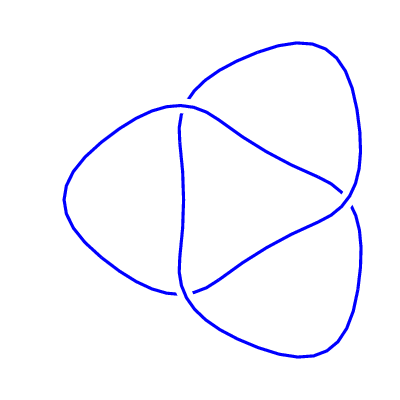
\includegraphics[width=\linewidth]{../data/3_1.png}
        \subcaption{$3_1$}
    \end{minipage}
    \begin{minipage}[b]{.14\linewidth}
        \centering
        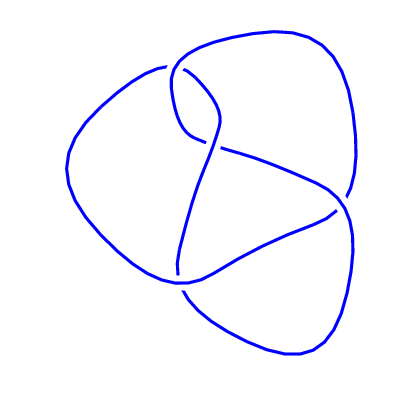
\includegraphics[width=\linewidth]{../data/4_1.png}
        \subcaption{$4_1$}
    \end{minipage}
    \begin{minipage}[b]{.14\linewidth}
        \centering
        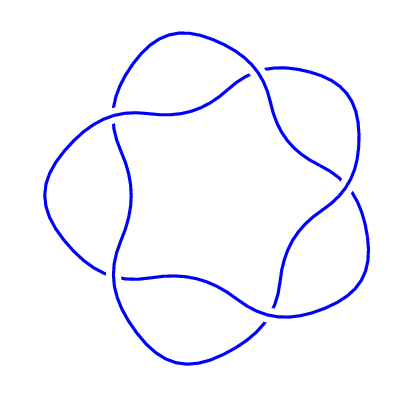
\includegraphics[width=\linewidth]{../data/5_1.png}
        \subcaption{$5_1$}
    \end{minipage}
    \begin{minipage}[b]{.14\linewidth}
        \centering
        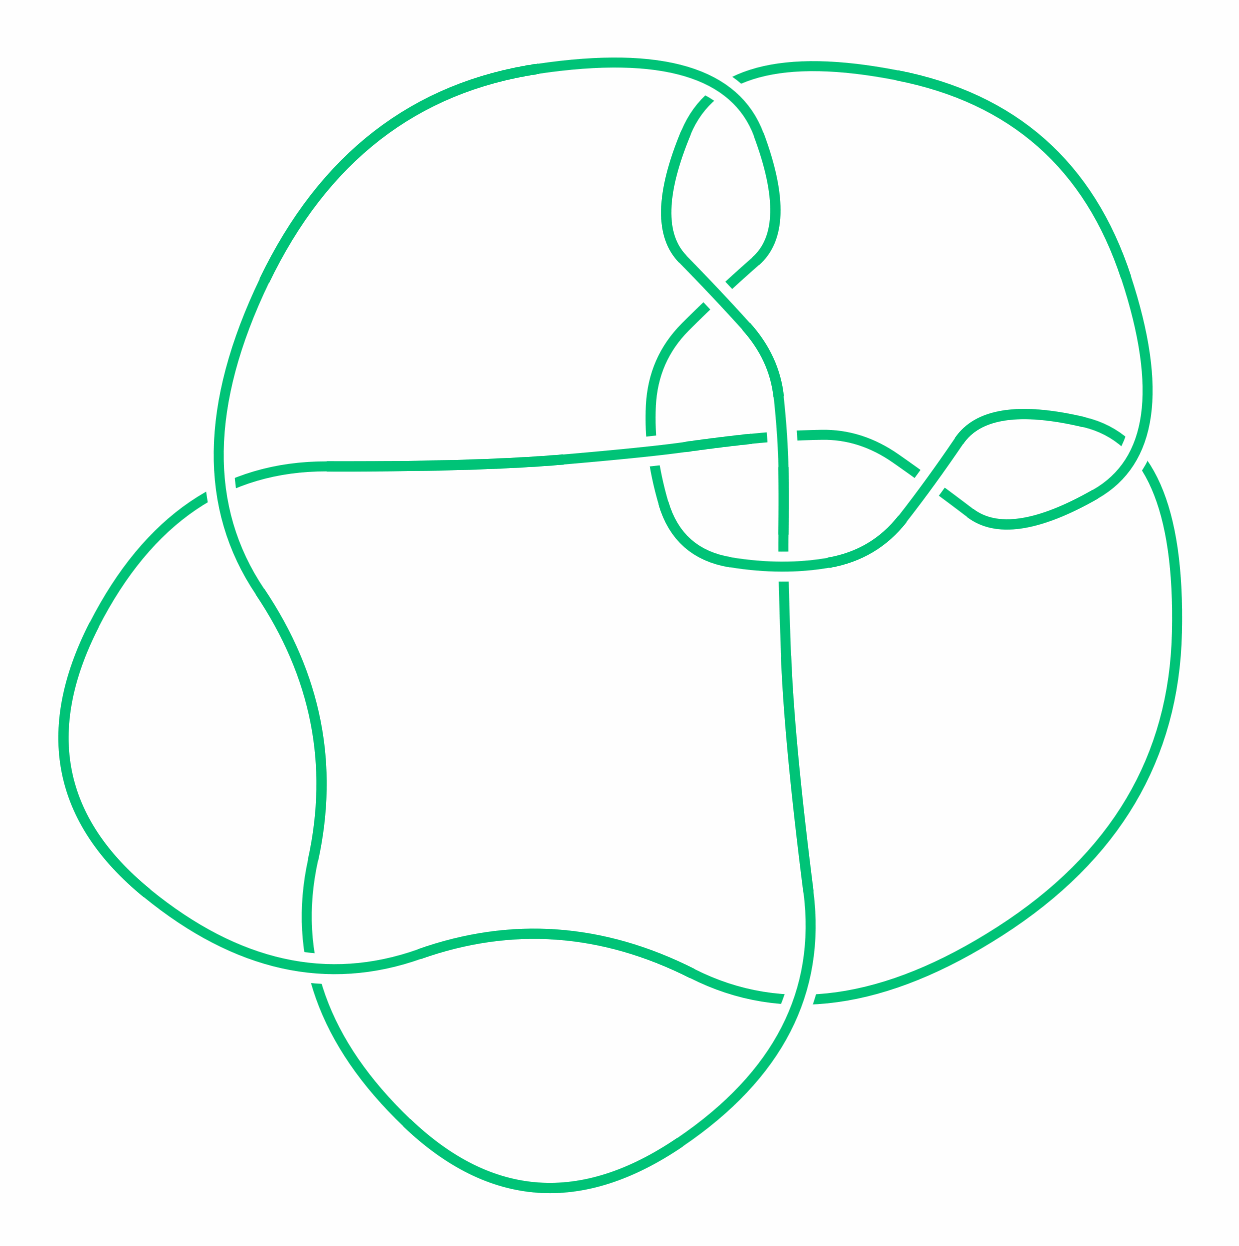
\includegraphics[width=\linewidth]{../data/perko1.png}
        \subcaption{$10_{161}$}
    \end{minipage}
    \begin{minipage}[b]{.14\linewidth}
        \centering
        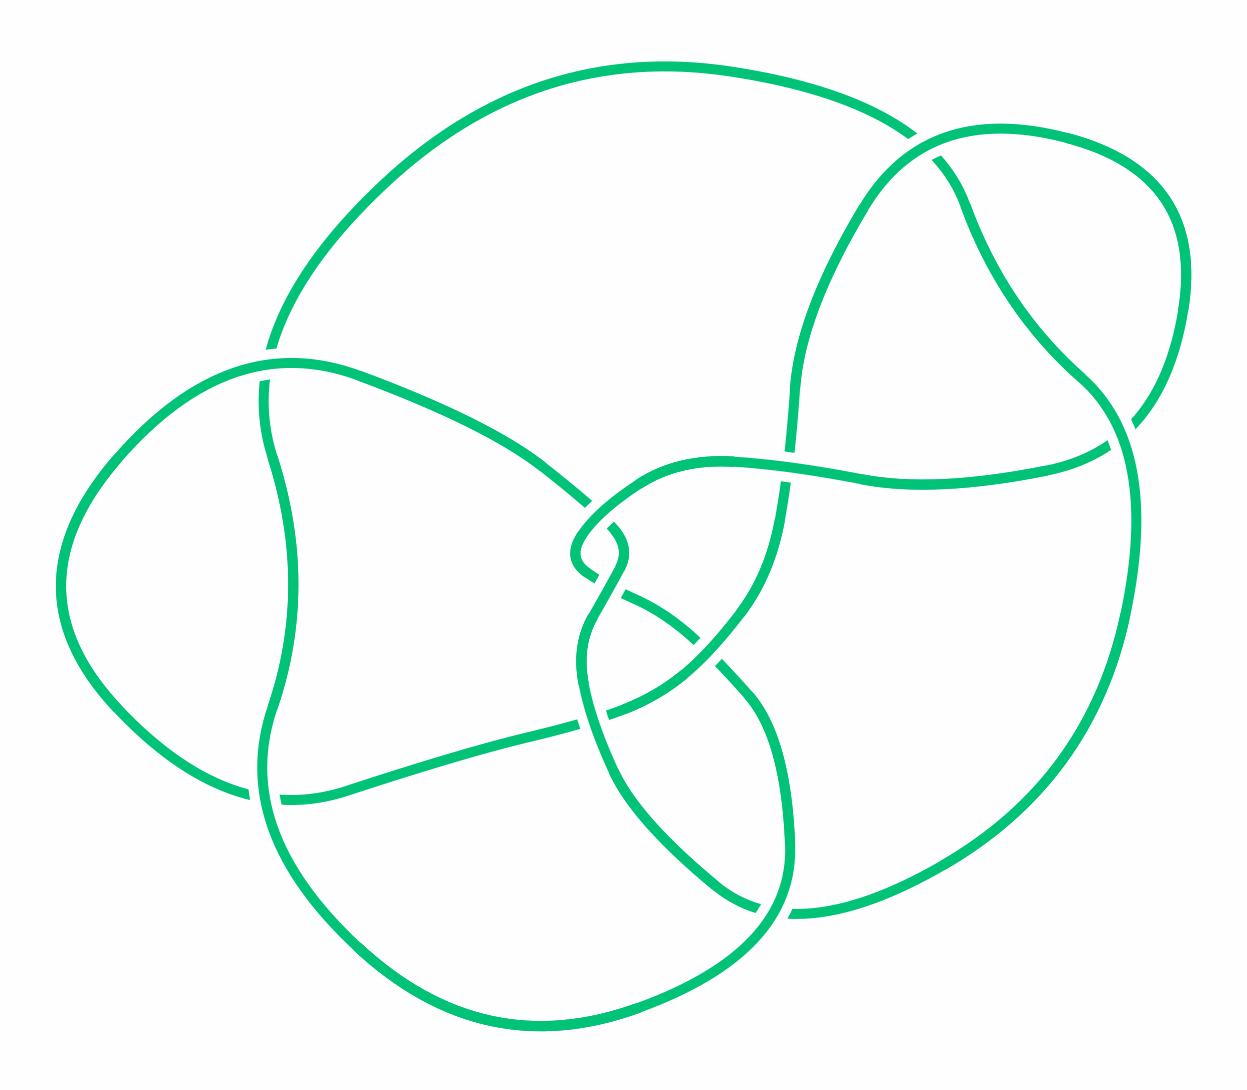
\includegraphics[width=\linewidth]{../data/perko2.png}
        \subcaption{$10_{162}$}
    \end{minipage}
\end{figure}

Początkowo celem teorii węzłów była klasyfikacja wszystkich węzłów.
Od XIX wieku, kiedy teoria węzłów wyodrębniła się jako osobny dział matematyki,
zdążyliśmy skatalogować ponad sześć miliardów tych obiektów.
Pozornie tak samo wyglądające węzły mogą się od siebie różnić.
Do wykrywania tych subtelnych różnic używa się przede wszystkim niezmienników topologicznych takich jak grupy, wielomiany bądź liczby.
Poznamy je w~dalszych rozdziałach.

Matematycy uogólnili pojęcie węzła:
można rozpatrywać je w~wyższych wymiarach albo zastąpić okrąg inną przestrzenią topologiczną.
Będziemy starać się unikać tych uogólnień.

\section{Węzły i~sploty}
Największą różnicą między węzłami matematycznymi oraz tymi z~prawdziwego jest życia jest to, że te pierwsze nie mają luźnych końców.
Można przyjąć nieidealną, naiwną definicję:

\begin{definition}[węzeł]
    Ciągłe oraz różnowartościowe odwzorowanie $S^1 \to \R^3$ nazywamy węzłem.
\end{definition}

Niestety, dopuszcza ona patologiczne z~kombinatorycznego punktu widzenia węzły dzikie, jak ten z~rysunku \ref{wild_knot}:

\begin{figure}
    \centering
    \label{wild_knot}
    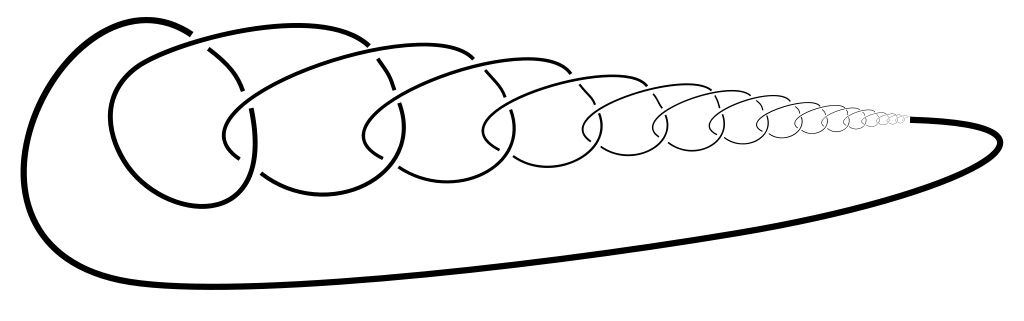
\includegraphics[width=0.5\linewidth]{wild_knot.png}
    \caption{Węzeł dziki}
\end{figure}

Zastanówmy się, jakim formalizmem opisać manipulowanie fizycznym sznurkiem, by wykluczyć węzły dzikie z~naszych rozważań.
Nie można użyć izotopii (dwa węzły są izotopijne, jeśli istnieje ciągła funkcja $F \colon S^1 \times [0, 1] \to \R^3$ taka, że $F(-, 0)$ jest pierwszym, zaś $F(-,1)$ drugim węzłem), gdyż każdy węzeł jest izotopijny z punktem:

{\color{red}\textbf{Tu brakuje obrazka.}}

W podobny sposób moglibyśmy przekształcić dowolny węzeł w~niewęzeł.
Teoria, w~której wszystkie obiekty są takie same, nie jest zbyt ciekawa.
Zwykła izotopia nie oddaje dobrze tego, czym jest równoważność węzłów wykonanych z~prawdziwego sznurka.
Trzeba od niej wymagać dodatkowo, by była gładka albo lokalnie płaska.
Z twierdzenia o rozszerzaniu izotopii wynika, że można ją wtedy podnieść do izotopii otaczającej.
Ta ostatnia uwzględnia, jak węzeł leży w~przestrzeni i okazuje się być właściwym pojęciem równości dla teorii węzłów:

\begin{definition}[izotopia otaczająca] \label{def_ambient_isotopy}
    Niech $N, M$ będą rozmaitościami, zaś $K_1, K_2 \colon N \to M$ włożeniami.
    Ciągłe odwzorowanie $F \colon M \times [0,1] \to M$ spełniające następujące warunki:
    \begin{enumerate}
        \item funkcja $F(-, 0)$ jest odwzorowaniem tożsamościowym,
        \item każda z funkcji $F(-, t)$ jest homeomorfizmem,
        \item złożenie $F(-, 1)$ z pierwszym włożeniem $K_1$ daje drugie włożenie $K_2$
    \end{enumerate}
    nazywamy izotopią otaczającą przenoszącą $K_1$ na $K_2$.
\end{definition}

W topologii rozważa się włożenia dowolnych rozmaitości, nam wystarczy jeden szczególny przypadek $N = S^1$ oraz $M = \R^3$.
Intuicyjnie, funkcja $F$ zniekształca przestrzeń $\R^3$ tak, że w~chwili początkowej $t = 0$ widzimy pierwszy, zaś w~chwili końcowej $t = 1$ drugi węzeł.
Izotopia otaczająca nie pozwala na ściąganie zaplątanych fragmentów do punktu.

{\color{red}\textbf{Homeomorfizmy $F_t$ można zastąpić przez dyfeomorfizmy zachowujące orientację. ???}}

\begin{definition}[węzeł]
    \label{def:knot}
    \index{węzeł}
    Gładkie włożenie $S^1 \to \R^3$ otaczająco izotopijne z~zamkniętą łamaną bez samoprzecięć nazywamy węzłem poskromionym.
\end{definition}

Przez prawie całą książkę interesować nas będą jedynie węzły poskromione,
dlatego jeśli nie zaznaczono inaczej, przez węzeł rozumiemy węzeł poskromiony.
Istnieje jeszcze jedna, konkurencyjna definicja węzłów równoważnych:

\begin{proposition}
    \label{equivalent_knots_2}
    Dwa węzły są równoważne, gdy jeden z~nich jest obrazem drugiego przez zachowujący orientację homeomorfizm $\R^3 \to \R^3$.
\end{proposition}

Stwierdzenie to przestaje być prawdziwe po zastąpieniu przestrzeni $\R^m$ przez $S^m$.

\begin{proof}
    Podany niżej dowód pochodzi z~książki ,,Topology from the differentiable viewpoint'' Johna Milnora.
    Musimy pokazać, że dyfeomorfizm $f \colon \R^m \to \R^m$ jest gładko izotopijny z~identycznością.
    Translacje są izotopiami, więc bez straty ogólności zakładamy, że $f(0) = 0$.
    Pochodna $f$ w~zerze jest dana wzorem $\mathrm{d}f_0(x) = \lim_{t \to 0} f(tx) /t$,
    naturalną definicję izotopii $F \colon \R^m \times [0, 1] \to \R^m$ stanowi więc
    \[
        F(x, t) = \begin{cases}
            \mathrm{d}f_0(x) & t = 0 \\
            f(tx) / t & 0 < t \le 1
        \end{cases} .
    \]

    Funkcja $F$ jest gładka, gdyż na mocy lematu Hadamarda funkcja $f$ zapisuje się jako suma $x_1 g_1(x) + \ldots + x_mg_m(x)$,gdzie funkcje $g_i$ są gładkie, co jakoś kończy dowód.
\end{proof}

Formalnie węzły to pewne odwzorowania, więc prawidłowym sposobem na zapisanie, że są izotopijne (czyli dla nas: równe), jest $K_1 \simeq K_2$.
Ponieważ nie prowadzi to do problemów, będziemy jednak stosować zapis $K_1 = K_2$.
Jednocześnie często węzeł (jako odwzorowanie) nie będzie odróżniany od obrazu tego odwzorowania.

\begin{definition}[splot, ogniwo]
    \label{def_link}
    \index{splot}
    Sumę parami rozłącznych węzłów $K_1, K_2, \ldots, K_n$ nazywamy splotem.
    Składniki sumy nazywamy ogniwami.
\end{definition}

Przez analogię do węzłów mówimy, że dwa sploty są takie same, jeśli jeden jest obrazem drugiego przez zachowujący orientację homeomorfizm $\R^3 \to \R^3$.
W~takiej sytuacji obydwa sploty mają tyle samo ogniw.

\begin{example}
    \index{splot!Hopfa}
    Splot Hopfa to najprostszy splot nietrywialny, którym w~1931 r. zajmował się Heinz Hopf, topolog niemiecki, w~ramach badań nad tzw. rozwłóknieniem (Hopf fibration).
    Whitehead w~1934 odkrył kontrprzykład do nieudanego dowodu hipotezy Poincarego.
    Był nim splot o~dwóch składowych przedstawiony na poniższym rysunku.

    \begin{figure}[H]
        \begin{minipage}[b]{.48\linewidth}
            \centering
            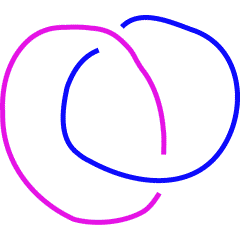
\includegraphics[width=0.5\linewidth]{../data/mixed/L2a1.png}
            \subcaption{splot Hopfa}
        \end{minipage}
        \begin{minipage}[b]{.48\linewidth}
            \centering
            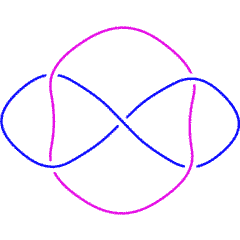
\includegraphics[width=0.5\linewidth]{../data/mixed/L5a1.png}
            \subcaption{splot Whiteheada}
        \end{minipage}
    \end{figure}
\end{example}

Jeśli dwa węzły są równoważne, to ich dopełnienia są oczywiście homeomorficzne.
Pytanie o~prawdziwość implikacji odwrotnej jako pierwszy zadał najprawdopodobniej w~1908 roku Tietze (,,Über die topologischen Invarianten mehrdimensionaler Mannigfaltigkeiten'').
W roku 1987 pokazano, że istnieją co najwyżej dwa węzły o~zadanym dopełnieniu (\cite{culler87}).
Dwa lata później poznaliśmy pozytywną odpowiedź na pytanie Tietzego: każdy węzeł jest wyznaczony jednoznacznie przez swoje dopełnienie.

\begin{theorem}[Gordon, Luecke, 1989]
    \label{thm_gordon_luecke}
    \index{twierdzenie!Gordona-Lueckego}
    Poskromione węzły o~homeomorficznych (z zachowaniem orientacji) dopełnieniach są wzajemnie izotopijne.
\end{theorem}

\begin{proof}[Niedowód]
    Wynika to z~ogólniejszego stwierdzenia:
    nietrywialna chirurgia Dehna na węźle w~3-sferze nigdy nie daje 3-sfery.
    Pełny dowód zawiera praca \cite{gordon89}.
\end{proof}

Twierdzenie to zamienia problem lokalny (czy dwa węzły w kuli $S^3$ są równoważne?) w~problem globalny (czy dwie przestrzenie topologiczne są homeomorficzne?).
Whitehead w~pracy \cite{whitehead37} z~1937 roku podał nieskończenie wiele splotów, których dopełnienia wyglądają jak dopełnienia splotu Whiteheada.
Odpowiednik twierdzenia \ref{thm_gordon_luecke} dla splotów jest więc fałszywy.

Poniższa definicja nie jest nam jeszcze potrzebna, ale wygodnie przytoczyć ją już teraz.

\begin{definition}[rozszczepialność]
    \index{splot!rozszczepialny}
    Jeżeli splot $L$ można zanurzyć w przestrzeni $\R^3$ tak, że niektóre jego ogniwa będą leżeć nad pewną rozłączną ze splotem płaszczyzną, zaś pozostałe pod nią, to powiemy, że splot $L$ jest rozszczepialny.
\end{definition}

Liczbę nierozszczepialnych splotów, pierwszych lub złożonych, zebrano w tabeli.
Źródło: baza danych OEIS, ciąg \href{https://oeis.org/A086825}{A086825}.

\renewcommand*{\arraystretch}{1.4}
\footnotesize
\begin{longtable}{lccccccccc}
    \hline
    \textbf{skrzyżowania}  &  0  &  1  &  2  &  3  &  4  &  5  &  6   &  7   &  8   \\  \hline  \endhead
    sploty                 &  1  &  0  &  1  &  1  &  3  &  4  &  15  &  24  &  82  \\
    \hline
\end{longtable}
\normalsize

\section{Diagramy. Ruchy Reidemeistera}
Chociaż w~świetle definicji \ref{def:knot} węzły są pewnymi regularnymi podzbiorami przestrzeni $\R^3$,
z kombinatorycznego punktu widzenia wygodniej jest rysować je na płaszczyźnie.

\begin{definition}[orientacja]
    \index{węzeł!zorientowany}
    Węzeł, w~którym wybrano kierunek, w~którym należy się po nim poruszać, nazywamy zorientowanym.
\end{definition}

\begin{definition} [diagram] \label{def_diagrams}
    \index{diagram}
    Cień to rzut węzła $K \subseteq \R^3$ na płaszczyznę.
    Cień razem z~informacją o~tym, jak przebiegają skrzyżowania i pozbawiony katastrof: potrójnych przecięć, stycznych czy dziobów nazywamy diagramem.
\end{definition}

{\color{red}\textbf{Narysować katastrofy}}

\begin{definition} [włókno]
    \index{włókno}
    Fragment diagramu, który biegnie między dwoma kolejnymi tunelami, czyli podskrzyżowaniami, nazywamy włóknem.
\end{definition}

\begin{definition} [nić]
    \index{nić}
    Fragment diagramu, który biegnie między dwoma kolejnymi skrzyżowaniami nazywamy nicią.
\end{definition}

Nici powstają z włókien przez rozcięcie ich przy każdym nadskrzyżowaniu.

\begin{proposition}
    Niech $K$ będzie węzłem.
    Zbiór diagramów jest otwarty i~gęsty w~zbiorze wszystkich rzutów.
\end{proposition}

\begin{proof}
    Rzut splotu na równoległe płaszczyzny jest taki sam, a te można sparametryzować prostymi przechodzącymi przez początek układu współrzędnych, które tworzą przestrzeń rzutową $\R \mathbb P^2$.
    Niech $S$ będzie zbiorem prostych, które dają złe rzuty.
    Wystarczy pokazać jego nigdziegęstość.
    Okazuje się, że $S$ jest też jednowymiarowy.
    (Dowód za \cite{crowell63}).
\end{proof}

Wynika stąd, że każdy węzeł ma wiele diagramów.
Mając dane dwa różne diagramy chcielibyśmy wiedzieć, czy reprezentują ten sam węzeł.
Na szczęście Reidemeister w latach 20. XX wieku podał proste kryterium rozstrzygające ten problem.
Najpierw zdefiniujmy trzy lokalne operacje na diagramach.

\begin{definition}
    \index{ruchy Reidemeistera}
    Trzy ruchy Reidemeistera, $R_1$, $R_2$, oraz $R_3$, to następujące deformacje diagramu:
    \[
        \underbrace{\begin{tikzpicture}[baseline=-0.65ex,scale=0.1]
        \begin{knot}[clip width=5]
            \strand[thick] (-5, 10) to [in=left, out=down] (2, -5);
            \strand[thick] (5, 0) to [in=right, out=down] (2, -5);
            \strand[thick] (5, 0) to [in=right, out=up] (2, 5);
            \strand[thick] (-5, -10) to [in=left, out=up] (2, 5);
        \end{knot}
        \end{tikzpicture}
        \, \cong \,
        \begin{tikzpicture}[baseline=-0.65ex,scale=0.1]
        \begin{knot}[clip width=5]
            \strand[thick] (0,10) to (0,-10);
        \end{knot}
        \end{tikzpicture}}_{R_1}
        %%%
        \quad \quad \quad
        \underbrace{\begin{tikzpicture}[baseline=-0.65ex,scale=0.1]
        \begin{knot}[clip width=5]
            \strand[thick] (-5, 10) to [in=up, out=down] (5, 0);
            \strand[thick] (-5, -10) to [in=down, out=up] (5, 0);
            \strand[thick] (5, 10) to [in=up, out=down] (-5, 0);
            \strand[thick] (5, -10) to [in=down, out=up] (-5, 0);
        \end{knot}
        \end{tikzpicture}
        \, \cong \,
        \begin{tikzpicture}[baseline=-0.65ex,scale=0.1]
        \begin{knot}[clip width=5]
            \strand[thick] (-5, 10) to [in=up, out=down] (-2, 0);
            \strand[thick] (-5, -10) to [in=down, out=up] (-2, 0);
            \strand[thick] (5, 10) to [in=up, out=down] (2, 0);
            \strand[thick] (5, -10) to [in=down, out=up] (2, 0);
        \end{knot}
        \end{tikzpicture}}_{R_2}
        %%%
        \quad \quad \quad
        \underbrace{\begin{tikzpicture}[baseline=-0.65ex,scale=0.1]
        \begin{knot}[clip width=5, flip crossing/.list={1,2,3}]
            \strand[thick] (-10, -10) -- (10, 10);
            \strand[thick] (-10, 10) -- (10, -10);
            \strand[thick] (-10, 0) to [in=left, out=right] (0, 10);
            \strand[thick] (10, 0) to [in=right, out=left] (0, 10);
        \end{knot}
        \end{tikzpicture}
        \, \cong \,
        \begin{tikzpicture}[baseline=-0.65ex,scale=0.1]
        \begin{knot}[clip width=5, flip crossing/.list={1,2,3}]
            \strand[thick] (-10, -10) -- (10, 10);
            \strand[thick] (-10, 10) -- (10, -10);
            \strand[thick] (-10, 0) to [in=left, out=right] (0, -10);
            \strand[thick] (10, 0) to [in=right, out=left] (0, -10);
        \end{knot}
        \end{tikzpicture}}_{R_3}
    \]
\end{definition}

Ruch $R_i$ operuje więc na $i$ łukach diagramu.
Reidemeister w~swojej pierwszej pracy przyjął inną kolejność,
jego drugi ruch jest naszym pierwszym.

\begin{theorem}[Reidemeister, 1927]
    \label{thm:reidemeister}
    Każdy splot posiada diagram.
    Dwa diagramy przedstawiają równoważne sploty,
    wtedy i~tylko wtedy gdy pierwszy można otrzymać z~drugiego
    wykonując skończenie wiele ruchów Reidemeistera
    oraz gładko deformując łuki bez zmiany biegu skrzyżowań.
\end{theorem}

Twierdzenie Reidemeistera jest prawdziwe zarówno dla splotów zorientowanych jak i~takich, które nie posiadają orientacji.

\begin{proof}
    Szkielet dowodu można znaleźć w~książce Burdego i~Zieschanga.
    Kluczowe pomysły zawiera ,,Knots, links, braids and $3$-manifolds''
    Prasołowa i~Sosińskiego.
    Innym przystępnym źródłem jest podręcznik \cite{murasugi96} Murasugiego ,,Knot theory and its applications''.
\end{proof}

{\color{red}\textbf{Brakuje prawdziwych cytowań}}

W praktyce twierdzenia \ref{thm:reidemeister} nie stosuje się bezpośrednio do diagramów splotów.
Jednym z~powodów jest wynik Cowarda i~Lackenby'a (\cite{coward11}): jeśli na dwóch diagramach tego samego węzła widać łącznie $n$ skrzyżowań, to ,,wystarcza''
\[
    R(n) = 2^{2^{\ldots^{2^n}}}
\]
ruchów Reidemeistera, by przejść między nimi; piętrowa potęga ma $10^{1000000n}$ warstw.
Gdy jeden z~diagramów jest pozbawiony skrzyżowań, czyli przedstawia niewęzeł, wystarcza $(236n)^{11}$ ruchów.
Zapewne lepsze ograniczenia istnieją, ale ich nie znamy.
Ważne jest to, że wielkość $R(n)$ jest skończona.

{\color{red}\textbf{Przedstawić rozumowanie (piramidka z węzłami), dlaczego to nie jest takie oczywiste.}}

Zamiast tego definiuje się niezmienniki, czyli funkcje ze zbioru wszystkich diagramów, które nie zmieniają swojej wartości podczas wykonywania ruchów Reidemeistera.
Kiedy pewien niezmiennik przyjmuje różne wartości na dwóch diagramach, te przedstawiają dwa istotnie różne sploty.
Gdy wartości są te same, nie dostajemy żadnej informacji.
Sploty mogą być równoważne albo nie.
Niezmienniki będą nam stale towarzyszyć w~wędrówce po krainie węzłów.

% koniec sekcji Ruchy Reidemeistera

%Niestety pomimo upływu czasus, nikt nie napisał komputerowego programu realizującego ten algorytm (stan na 1994).
%Może podejmie się tego Czytelnik?
%Inne algorytmy istnieją, jednak wszystkie działają w~wykładniczym czasie.

W 1961 roku W. Haken \cite{haken61} podał niezawodny przepis na wykrycie diagramu niewęzła,
częściowo rozwiązując jeden z~ważniejszych problemów teorii węzłów.
Przez wiele lat nikt nie podjął się implementacji tego algorytmu,
udało się to niedawno Burtonowi, Budneyowi oraz Petterssonowi w~komputerowym programie Regina\footnote{Dostępny pod adresem \url{https://regina-normal.github.io/}.} na przełomie tysiącleci.
Burton, Rubinstein i~Tillman pokazali w~pracy \cite{burton12}, jak sprawdzać,
czy powierzchnia normalna na striangulowanej 3-rozmaitości jest (nie)ściśliwa w~czasie wykładniczym.
To okazało się być wystarczającym do udzielenia negatywnej odpowiedzi na pytanie Thurstona:
,,czy przestrzeń Seiferta-Webera jest rozmaitością Hakena?'',
a zatem wykraczającego poza poziom tej pracy.
Patrz także {\url{http://geometrygames.org/SnapPea/index.html}.

{\color{red}\textbf{Dowiązać tutaj wszystkie wykrywacze niewęzła opisane w książce}}

Przykładami trudnych w~rozpoznaniu niewęzłów są: niewęzeł Goritza, Freedmana.
Więcej trudnych niewęzłów zawiera praca \cite{zanellati16} autorstwa C. Petronio oraz A. Zanellatiego.

\begin{figure}[H]
    \begin{minipage}[b]{.32\linewidth}
        \centering
        
\includegraphics[width=\linewidth]{../data/missing.jpg}
        \subcaption{normalny}
    \end{minipage}
    \begin{minipage}[b]{.32\linewidth}
        \centering
        
\includegraphics[width=\linewidth]{../data/missing.jpg}
        \subcaption{Goritza}
    \end{minipage}
    \begin{minipage}[b]{.32\linewidth}
        \centering
        
\includegraphics[width=\linewidth]{../data/missing.jpg}
        \subcaption{Freedmana}
    \end{minipage}
\end{figure}

Zanim opowiemy, jak dotąd przebiegała klasyfikacja węzłów o małej liczbie skrzyżowań, zdefiniujemy klasę splotów ze specjalnymi diagramami.

\begin{definition}[alternacja]
    \index{węzeł!alternujący}
    Diagram splotu, gdzie podczas poruszania się wzdłuż każdego ogniwa nad- oraz podskrzyżowania mijane są naprzemiennie, nazywamy alternującym.
    Splot jest alternujący, jeśli posiada alternujący diagram.
\end{definition}

Około 1961 roku Fox zapytał ,,What is an alternating knot?''.
Szukano takiej definicji węzła alternującego, która nie odnosi się bezpośrednio do diagramów, aż w~2015 roku Joshua Greene podał geometryczną charakteryzację: nierozdzielczy splot w $S^3$ jest alternujący wtedy i tylko wtedy, gdy ogranicza dodatnią oraz ujemną określoną powierzchnię rozpinającą \cite{greene17}.
% definite spanning surface

Sundberg oraz Thistlethwaite pokazali w 1998 roku, że liczba splotów alternujących rośnie wykładniczo (\cite{sundberg98}):

\begin{proposition}
    Niech $a_n$ oznacza liczbę pierwszych, alternujących supłów o~$n$ skrzyżowaniach.
    Wtedy
    \begin{equation}
        a_n \sim (3c_1/4\sqrt{\pi})n^{-5/2}\lambda^{n-3/2},
    \end{equation}
    gdzie zarówno $c_1$, pierwszy współczynnik rozwinięcia Taylora funkcji $\Phi(\eta)$ zdefiniowanej w \cite{sundberg98}, jak i $\lambda$ są jawnie znanymi stałymi:
    \begin{align}
        c_1 & = \sqrt{\frac{5^7 \cdot (21001 + 371 \sqrt{21001})^3}{2 \cdot 3^{10} \cdot (17 + 3\sqrt{21001})^5}} \\
        \lambda & = \frac {1}{40} (101 + \sqrt{21001})
    \end{align}
    Niech $A_n$ oznacza liczbę pierwszych, alternujących splotów o $n$ skrzyżowaniach.
    Wtedy $A_n \approx \lambda^n$, dokładniej: jeśli $n \ge 3$, to
    \begin{equation}
        \frac{a_{n-1}}{16n - 24} \le A \le \frac{a_n - 1}{2}.
    \end{equation}
\end{proposition}

Czasami będziemy używać słów przed ich zdefiniowaniem, tak jak uczyniliśmy tutaj: węzły pierwsze i~supły pojawiają się odpowiednio w definicjach \ref{primeknot}, \ref{def:tangle}.
Książkę trzeba więc przeczytać co~najmniej dwa razy.

\begin{proposition}
    Niech $a_n$ oznacza liczbę pierwszych, alternujących supłów o~$n$ skrzyżowaniach.
    Wtedy funkcja tworząca $f(z) = \sum_n a_n z^n$ spełnia równanie
    \begin{equation}
    f(1+z) - f(z)^2 - (1+f(z))q(f(z)) -z - \frac{2z^2}{1-z} = 0,
    \end{equation}
    gdzie $q(z)$ jest pomocniczą funkcją
    \begin{equation}
        q(z) = \frac{2z^2 - 10z - 1 + \sqrt{(1-4z)^3}} {2(z+2)^3} - \frac{2}{1+z} -z + 2.
    \end{equation}
\end{proposition}

Fakt ten stanowi raczej ciekawostkę i także pochodzi z cytowanej wcześniej pracy \cite{sundberg98}.

\subsection{Historia tablic węzłów}
Pierwszą osobą, która podjęła się szukania węzłów, był Peter Guthrie Tait, szkocki fizyk.
Razem z Thomsonem (lordem Kelvinem) wierzyli, że węzły są kluczem do zrozumienia widma spektroskopowego różnych pierwiastków: na przykład atom sodu mógł być splotem Hopfa ze względu na dwie linie emisyjne.
Eksperyment Michelsona-Morleya z 1887 roku zabił ich ,,wirową teorię atomu'', ale nie miało to znaczenia dla teorii węzłów jako działu matematyki.

Używana po dziś dzień strategia, którą przyjął Tait, jest stosunkowa prosta: narysować wszysktie możliwe diagramy o~zadanym indeksie skrzyżowaniowym, po czym połączyć ze sobą te, które przedstawiają jeden węzeł.
Na potrzeby pierwszego etapu Tait wymyślił schemat kodowania diagramów.
Wiele lat wcześniej, Gauss wraz ze swoim uczniem Listingiem badał węzły i~opracował (niezależnie!) podobną notację.
My przytoczymy opis dalszego ulepszenia tej metody, zwanego notacją Dowkera-Thistletwaite’a.

Tait wykorzystując swoją notację podał w~1876 pierwszą tablicę piętnastu węzłów o~mniej niż ośmiu skrzyżowaniach.
Nie należy traktować tego jako skromny wynik: nie miał on do dyspozycji żadnych twierdzeń topologicznych do odróżniania węzłów.
Onieśmielony przez liczbę możliwych ciągów dla kolejnych indeksów skrzyżowaniowych, powstrzymał się przed rozszerzaniem swojej tablicy.
To właśnie grupowanie diagramów przedstawiających ten sam węzeł, a~nie samo szukanie wszystkich możliwych diagramów, sprawia trudność.

Aby sobie pomóc, Tait znalazł lokalną modyfikację diagramu, która nie zmienia indeksu skrzyżowaniowego, znaną obecnie jako flype.

\[
\begin{tikzpicture}[baseline=-0.65ex, scale=0.1]
\begin{knot}[clip width=5, end tolerance=1pt, flip crossing/.list={1}]
    \strand[semithick] (-21, -5) [in=180, out=0] to (-7, 5);
    \strand[semithick] (-21, 5) [in=180, out=0] to (-7, -5);
    \draw (-7, -7) rectangle (7, 7);
    \node at (0, 0) {\Huge {$T$}};
    \draw[semithick] (7, -5) to (21, -5);
    \draw[semithick] (7, 5) to (21, 5);
\end{knot}
\end{tikzpicture}
\quad \cong_{\mathrm{flype}} \quad
\begin{tikzpicture}[baseline=-0.65ex, scale=0.1]
\begin{knot}[clip width=5, end tolerance=1pt]
    \strand[semithick] (21, -5) [in=0, out=180] to (7, 5);
    \strand[semithick] (21, 5) [in=0, out=180] to (7, -5);
    \draw (-7, -7) rectangle (7, 7);
    \node at (0, 0) {\rotatebox[origin=c]{-180}{\Huge $T$}};
    \draw[semithick] (-7, -5) to (-21, -5);
    \draw[semithick] (-7, 5) to (-21, 5);
\end{knot}
\end{tikzpicture}
\]

Inną taktykę szukania węzłów przyjał wielebny Thomas Kirkman: zaczynał od małego zbioru "nieredukowalnych" rzutów, do których systematycznie dokładał skrzyżowania.
Tait przeczytał pracę Kirkmana, po czym w~latach 1884/1885 opracował listę węzłów alternujących o~mniej niż 11 skrzyżowaniach.
Tuż przed oddaniem jej do druku odkrył inny spis węzłów stworzony przez amerykańskiego naukowca Charlesa Little'a.
Znalazł wtedy jeden duplikat u~siebie, natomiast u Little'a jeden duplikat i~jedno pominięcie.

Zachęcony przez Taita, Little zabrał się za alternujące węzły o~11 skrzyżowaniach i~za trudniejsze zadanie, stablicowanie węzłów niealternujących, czyli takich, które nie posiadają alternującego diagramu.
Jak wynika z~pierwszej pracy Taita, początkowo nie wierzono, że takie w~ogóle istnieją.
Dowód znaleziono wiele lat później, niealternujące są $8_{19}$, $8_{20}$, $8_{21}$, ale nie pierwsze węzły o mniejszej liczbie skrzyżowań.
Patrz twierdzenie \ref{prp:bankwitz}.
Little pracował przez sześć lat (1893 -- 1899) i~znalazł 43 niealternujące węzły o~10 skrzyżowaniach.
Żadnego nie pominął, ale trafił mu się jeden duplikat.

W kolejnych dziesięcioleciach nie nastąpił znaczący postęp, zarówno w~rozszerzaniu tablic jak i~sprawdzaniu tych już istniejących.
Haseman w~1918 roku znalazł achiralne węzły o~12 i~14 skrzyżowaniach.
W 1927 roku Alexander z~Briggsem przy użyciu pierwszej grupy homologii rozgałęzionego nakrycia cyklicznego (!) potrafili odróżnić od siebie dowolne dwa węzły (z~pominięciem trzech par) o~co najwyżej 9 skrzyżowaniach.
Reidemeister poradził sobie z~tymi wyjątkami w~1932 roku, korzystając z~indeksu zaczepienia i~homomorfizmów z~grupy węzła na grupy diedralne.
% branch curves in irregular covers associated to homomorphisms of the knot group onto dihedral groups

%%%%% Tait, Little wyprodukowali prawie bezbłędną tablicę węzłów o~co najwyżej 11 skrzyżowaniach przy użyciu grafów.

Dopiero Conway w~latach sześćdziesiątych minionego wieku znalazł pierwsze węzły o~mniej niż 12 skrzyżowaniach oraz wszystkie sploty o~mniej niż 11 skrzyżowaniach w~oparciu o~pomysły Kirkmana.
% An enumeration of knots and links, 1970.
Zajęło mu to jedynie kilka godzin!
Conway znalazł 1 duplikat oraz 11 pominięć w~tablicach Little'a, ale sam popełnił 4 pominięcia.
Przeoczył między innymi słynny duplikat w~niealternującej tablicy Little'a, parę Perko.
% 1974?
Przyczyną było prawdopodobnie to, że dwa diagramy miały różny spin:
Little błędnie twierdził, że spin minimalnego diagramu jest niezmiennikiem, gdyż błędnie założył, że flype oraz 2-przejścia wystarczają do zmiany jednego minimalnego diagramu w~inny.

Pominęcia w~tablicy Conwaya znalazł Caudron w~1980 roku.
Nieopublikowany manuskrypt Bonahona, Siebenmanna klasyfikuje węzły algebraiczne.
Z~nielicznymi niealgebraicznymi węzłami do 11 skrzyżowań poradził sobie Perko około 1980 roku (,,Invariants of 11-crossing knots'').
To był kres ery ręcznych obliczeń.

Na początku lat osiemdziesiątych Dowker i~Thistlethwaite stabularyzowali z~pomocą komputera węzły do 13 skrzyżowań.
Przez blisko dekadę nic się nie działo, aż grupa studentów wygrała dostęp do superkomputera Cray.
Razem z~Hoste znaleźli alternujące węzły do 14 skrzyżowań, jednocześnie sprawdzając istniejące tabele Thistlethwaite'a.
Około roku 1998 Hoste z~Weeksem (oraz niezależnie Thistlethwaite) znaleźli 1701936 pierwszych węzłów do 16 skrzyżowań.
Spośród nich, tylko 32 nie jest węzłami hiperbolicznymi, wszystkie pozostałe poddają się maszynerii geometrii hiperbolicznej.

\subsection{Hipotezy Taita}
\begin{conjecture}[I hipoteza Taita]
    \label{conj_tait_i}
    \index{hipoteza!Taita}
    Zredukowany alternujący diagram splotu ma minimalny indeks skrzyżowaniowy.
\end{conjecture}
% To bardzo ważny rezultat, którego prawdziwość przypuszczał już P. G. Tait w~XIX wieku.
% Nikt nie był w~stanie podać dowodu przed pojawieniem się wielomianu Jonesa.

Najpierw znaleziono dowód korzystający z wielomianu Jonesa (Kauffman \ref{kauffman87}, Murasugi \ref{murasugi87}, Thistlethwaite \ref{thistlethwaite87}, wszystkie prace z 1987 roku).
Trzydzieści lat później Greene zaprezentował geometryczne podejście do problemu w \ref{greene17}.

\begin{conjecture}[II hipoteza Taita]
    \label{conj_tait_ii}
    Achiralny splot alternujący ma zerowy spin.
\end{conjecture}

Pierwsze dowody pochodzą znowu od Kauffmana \ref{kauffman87} oraz Thistlethwaite'a \ref{thistlethwaite87}.

\begin{conjecture}[III hipoteza Taita]
    \label{conj_tait_iii}
    Niech $D_1, D_2$ będą zredukowanymi alternującymi diagramami zorientowanego pierwszego splotu.
    Wtedy diagram $D_2$ można otrzymać z~$D_1$ korzystając jedynie z~ruchu \emph{flype}.
\end{conjecture}

Tę hipotezę udowodnił Menasco z Thistlethwaitem, \ref{menasco91}.
Wynika z~niej, że dwa zredukowane diagramy alternujące tego samego węzła mają ten sam spin: ruch flype nie zmienia spinu (dla niektórych to jest II hipoteza).	
My pokażemy nieco później, czyli po poznaniu wielomianu Jonesa, że wszystkie trzy hipotezy są prawdziwe.

\textbf{Wstawić odniesienia do naszego dowodu}

\subsection{Metody kodowania}
\subsubsection{Notacja Alexandera-Briggsa}
Najbardziej tradycyjna, wprowadzona w~1927 roku, rozszerzona później przez Rolfsena.

\subsubsection{Notacja Dowkera-Thistlethwaite'a}
Poprawia notację Taita.
Należy ustalić minimalny diagram węzła, dowolny punkt początkowy oraz kierunek i zacząć przemierzać węzeł.
Za każdym razem, kiedy mijamy skrzyżowanie, przypisujemy mu kolejną liczbę naturalną, zaczynając od jedynki.
Jeżeli znajdujemy się nad skrzyżowaniem, parzyste etykiety zapisujemy z przeciwnym znakiem.
Kiedy skończymy, każde skrzyżowanie będzie mieć dwie etykiety.

\begin{definition}
	Ciąg parzystych liczb występujących na diagramie kolejno przy $1, 3, \ldots$ nazywamy kodem Dowkera-Thistlethwaite'a.
\end{definition}

Opisany powyżej kod nie jest idealny, ponieważ odtworzony z niego węzeł może być lustrzanym odbiciem wyjściowego.
Ogólniej, odbicie dowolnego składnika sumy spójnej nie zmienia kodu całego węzła.
Nie stanowi to jednak dużego problemu, ponieważ notacja została stworzona na potrzeby tablicowania węzłów pierwszych, a~te są niezorientowane.

Zaczynając od zredukowanego diagramu o $n$ skrzyżowaniach nie można doprowadzić do sytuacji, gdzie do pewnego skrzyżowania przypisane są dwie kolejne liczby całkowite.
Dzięki temu problem można przetłumaczyć na język teorii grafów.
Rozpatrzmy graf $G$, którego wierzchołkami są liczby $1, 2, \ldots, 2n$.
Połączmy niesąsiadujące modulo $2n$ wierzchołki o różnej parzystości krawędziami.
Graf ten powstaje przez usunięcie cyklu Hamiltona (łączącego kolejne liczby) z pełnego grafu dwudzielnego.
Zbiór par etykiet przy skrzyżowaniach węzła to skojarzenie doskonałe w grafie $G$.
Liczba skojarzeń prawie pokrywa się z rozwiązaniem zadania znanego w literaturze jako ,,problème des ménages'': na ile sposobów $n$ małżeństw można posadzić przy okrągłym stole tak, by żadne małżeństwo nie siedziało obok siebie i~każdy mężczyzna znalazł się obok dwóch kobiet?
Ustawienia, które powstają przez cykliczne permutowanie należy uznać za tożsame.
Gilbert znalazł w \cite{gilbert56} wzór na $a_n$, liczbę różnych kodów:
\begin{align}
u(m, t) & = 2m \sum_{k=0}^m {2m-k \choose k} \cdot (m-k)! \cdot \frac{(t-1)^k}{2m - k}  \\
a(n) & = \frac{1}{n} \sum_{d\mid n} \left(\frac{n}{d}\right)^d \cdot u \left(d, 1 - \frac{d}{n}\right) \cdot \varphi \left(\frac{n}{d}\right)
\end{align}

Kilka początkowych wartości to $a_3 = 1, 2, 5, 20, 87, 616, 4843, 44128, 444621, \ldots$ (ciąg A002484 w OEIS).

\subsubsection{Notacja Conwaya}
Wprowadzona przez Conwaya w~pracy \cite{conway70}.
Opiera się na pojęciu supła, dlatego więcej szczegółów przedstawiamy dopiero w definicji \ref{conway_notation}.

% A pictorial enumeration of prime knots of up to 10 crossings appears in Rolfsen (1976, Appendix C).
% Note, however, that in this table, the Perko pair 10-161 and 10-162 are actually identical, and the uppermost crossing in 10-144 should be changed (Jones 1987).

% Rolfsen's last four 10 crossing knots have been renumbered, to avoid the Perko duplication.
% A further mistake in Rolfsen's tables is that therein 1083 and 1086 were swopped: the Conway notation and Alexander polynomial for each one referred to the diagram of the other.
% We exchange not diagrams, but Alexander polynomial and Conway notation to fix the mistake (like the table in the new 2003 edition of the Rolfsen book, Dror Bar-Natan's Knot Atlas, and Chuck Livingston's Table of Knot Invariants, and unlike in Kawauchi's book!).
% http://stoimenov.net/stoimeno/homepage/ptab/

\section{Ruchy Reidemeistera}
\label{sec:reidemeister_moves}
W kombinatorycznej teorii węzłów diagramy są dużo ważniejsze od gładkich włożeń okręgu w przestrzeń $\R^3$,
dlatego przytoczymy proste kryterium decydujące o tym,
kiedy dwa diagramy przedstawiają jeden węzeł.
Najpierw zdefiniujmy trzy lokalne operacje na diagramach.

\begin{definition}
    Trzy ruchy Reidemeistera, $R_1$, $R_2$, oraz $R_3$, to następujące deformacje diagramu:
    \[
        \underbrace{\begin{tikzpicture}[baseline=-0.65ex,scale=0.1]
        \begin{knot}[clip width=5]
            \strand[thick] (-5, 10) to [in=left, out=down] (2, -5);
            \strand[thick] (5, 0) to [in=right, out=down] (2, -5);
            \strand[thick] (5, 0) to [in=right, out=up] (2, 5);
            \strand[thick] (-5, -10) to [in=left, out=up] (2, 5);
        \end{knot}
        \end{tikzpicture}
        \, \cong \,
        \begin{tikzpicture}[baseline=-0.65ex,scale=0.1]
        \begin{knot}[clip width=5]
            \strand[thick] (0,10) to (0,-10);
        \end{knot}
        \end{tikzpicture}}_{R_1}
        %%%
        \quad \quad \quad
        \underbrace{\begin{tikzpicture}[baseline=-0.65ex,scale=0.1]
        \begin{knot}[clip width=5]
            \strand[thick] (-5, 10) to [in=up, out=down] (5, 0);
            \strand[thick] (-5, -10) to [in=down, out=up] (5, 0);
            \strand[thick] (5, 10) to [in=up, out=down] (-5, 0);
            \strand[thick] (5, -10) to [in=down, out=up] (-5, 0);
        \end{knot}
        \end{tikzpicture}
        \, \cong \,
        \begin{tikzpicture}[baseline=-0.65ex,scale=0.1]
        \begin{knot}[clip width=5]
            \strand[thick] (-5, 10) to [in=up, out=down] (-2, 0);
            \strand[thick] (-5, -10) to [in=down, out=up] (-2, 0);
            \strand[thick] (5, 10) to [in=up, out=down] (2, 0);
            \strand[thick] (5, -10) to [in=down, out=up] (2, 0);
        \end{knot}
        \end{tikzpicture}}_{R_2}
        %%%
        \quad \quad \quad
        \underbrace{\begin{tikzpicture}[baseline=-0.65ex,scale=0.1]
        \begin{knot}[clip width=5, flip crossing/.list={1,2,3}]
            \strand[thick] (-10, -10) -- (10, 10);
            \strand[thick] (-10, 10) -- (10, -10);
            \strand[thick] (-10, 0) to [in=left, out=right] (0, 10);
            \strand[thick] (10, 0) to [in=right, out=left] (0, 10);
        \end{knot}
        \end{tikzpicture}
        \, \cong \,
        \begin{tikzpicture}[baseline=-0.65ex,scale=0.1]
        \begin{knot}[clip width=5, flip crossing/.list={1,2,3}]
            \strand[thick] (-10, -10) -- (10, 10);
            \strand[thick] (-10, 10) -- (10, -10);
            \strand[thick] (-10, 0) to [in=left, out=right] (0, -10);
            \strand[thick] (10, 0) to [in=right, out=left] (0, -10);
        \end{knot}
        \end{tikzpicture}}_{R_3}
    \]
\end{definition}

Ruch $R_i$ operuje więc na $i$ łukach diagramu.
Reidemeister w swojej pierwszej pracy przyjął innął kolejność,
jego drugi ruch jest naszym pierwszym.

\begin{theorem}[Reidemeister, 1927]
    Każdy splot posiada diagram.
    Dwa diagramy przedstawiają równoważne sploty,
    wtedy i tylko wtedy gdy pierwszy można otrzymać z drugiego
    wykonując skończenie wiele ruchów Reidemeistera
    oraz gładko deformując łuki bez zmiany biegu skrzyżowań.
\end{theorem}

\begin{proof}
    Szkielet dowodu można znaleźć w książce Burdego i Zieschanga.
    Kluczowe pomysły zawiera ,,Knots, links, braids and $3$-manifolds''
    Prasołowa i Sosinskiego.
    Innym przystępnym źródłem jest podręcznik \cite{murasugi96} Murasugiego ,,Knot theory and its applications''.
\end{proof}

Twierdzenie Reidemeistera jest użytecznym narzędziem,
z którego będziemy korzystać podczas definiowania większości niezmienników,
obiektów, które pozwalają odróżniać od siebie węzły.
Rzadko stosuje się je do przechodzenia między dwoma diagramami.
Istotnie, Coward i Lackenby udowodnili w \cite{coward11},
że jeśli dwa diagramy o $n$ skrzyżowaniach przedstawiają jeden węzeł, wystarcza
\[
    R(n) = 2^{2^{\ldots^{2^n}}}
\]
(gdzie piętrowa potęga ma $10^{1000000n}$ warstw) ruchów Reidemeistera, by przejść między nimi.
Jeśli jeden z diagramów jest pozbawiony skrzyżowań, wystarcza $(236n)^{11}$ ruchów.
Zapewne lepsze ograniczenia istnieją, ale ich nie znamy.
Ważne jest to, że wielkość $R(n)$ jest skończona.

\begin{definition}
    Węzeł zorientowany to taki, w którym wybrano kierunek, w którym należy się po nim poruszać.
\end{definition}

Twierdzenie Reidemeistera pozostaje prawdziwe dla węzłów zorientowanych.

% koniec sekcji Ruchy Reidemeistera

\section{Operacje na węzłach} % (fold)
W tej sekcji poznamy sposoby otrzymywania nowych obiektów z~już istniejących (rewers i~lustro splotu).
Rodzina węzłów wyposażona w~sumę spójną tworzy przemienny monoid z~jednoznacznością rozkładu.
Znacznie później (w sekcji \ref{sec:tangle}) określimy jeszcze sumę oraz iloczyn supłów.

\subsection{Lustro i~rewers} % (fold)
\begin{definition}[lustro]
    \index{lustro}
    \index{węzeł!lustrzany}
    Niech $L$ będzie zorientowanym splotem.
    Splot $mL$ powstały przez odbicie splotu $L$ względem dowolnej płaszczyzny nazywamy lustrem.
\end{definition}

\begin{definition}[rewers]
    \index{rewers}
    \index{węzeł!odwrotny}
    Niech $L$ będzie zorientowanym splotem.
    Splot $rL$ powstały przez odwrócenie orientacji wszystkich ogniw splotu $L$ nazywamy rewersem.
\end{definition}

\begin{comment}
\begin{figure}[H]
    \begin{minipage}[b]{.32\linewidth}
        \centering
        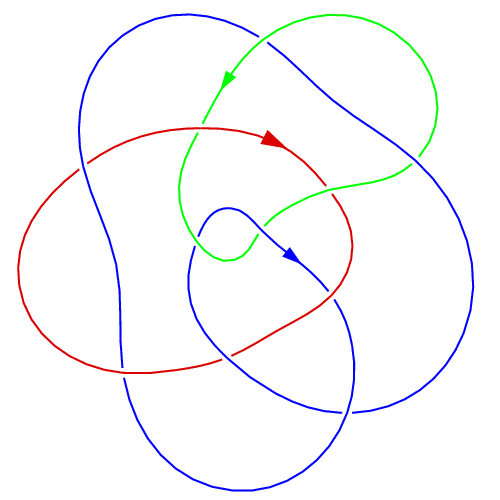
\includegraphics[width=\linewidth]{../data/link_mirror.png}
        \subcaption{lustro $mL$}
    \end{minipage}
    \begin{minipage}[b]{.32\linewidth}
        \centering
        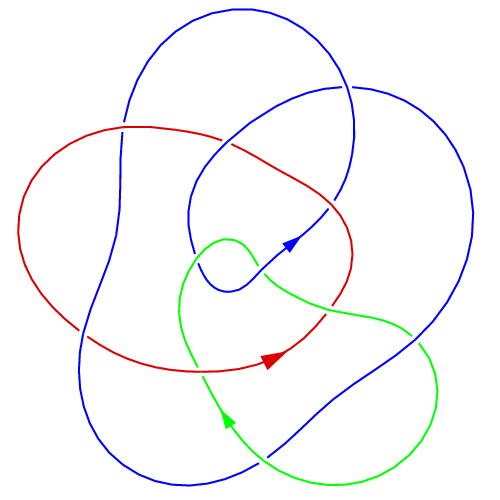
\includegraphics[width=\linewidth]{../data/link.png}
        \subcaption{przykładowy splot $L$}
    \end{minipage}
    \begin{minipage}[b]{.32\linewidth}
        \centering
        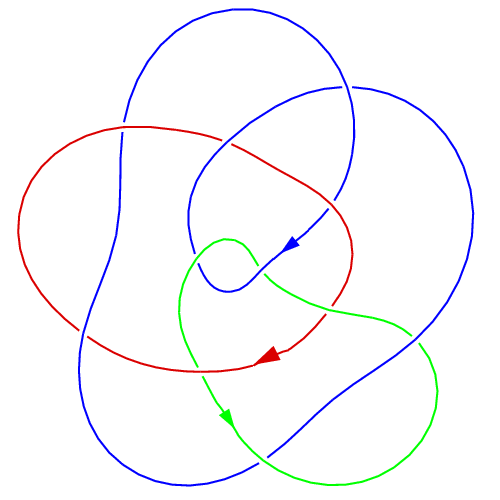
\includegraphics[width=\linewidth]{../data/link_reverse.png}
        \subcaption{rewers $rL$}
    \end{minipage}
\end{figure}
\end{comment}

Na lewym obrazku odbiliśmy diagram względem poziomej prostej, innym sposobem na otrzymanie lustra jest odwrócenie wszystkich skrzyżowań, co odpowiada odbijaniu względem płaszczyzny papieru.
Zauważmy, że wykonując powyższe operacje na węźle możemy otrzymać mniej niż czterech różne obiekty ($L$, $mL$, $rL$, $mrL$) -- na przykład trójlistnik jest własnym rewersem, ale nie lustrem.

Wyróżniamy pięć typów symetrii węzłów:

\begin{definition}[całkowicie chiralny albo skrętny]
    \index{węzeł!chiralny (skrętny)}
    Węzły $K$, $rK$, $mK$ są parami nierównoważne. % chiral 9_32
\end{definition}

\begin{definition}[odwracalny]
    \index{węzeł!odwracalny}
    Węzły $K \cong rK$ są równoważne. % reversible 3_1
\end{definition}

\begin{definition}[zwierciadlany ujemnie]
    \index{węzeł!zwierciadlany}
    Węzły $K \cong mrK$ są równoważne. % negative amphicheiral 8_17
\end{definition}

\begin{definition}[zwierciadlany dodatnio]
    Węzły $K \cong mK$ są równoważne. % positive amphicheiral 12a_427
\end{definition}

\begin{definition}[całkowicie zwierciadlany]
    Węzły $K, rK, mK$ są parami równoważne. % fully amphicheiral 4_1
\end{definition}

\begin{example}
    Węzeł $9_{32}$ jest całkowicie skrętny.
\end{example}

Całkowicie skrętne są też między innymi wszystkie węzły torusowe.

\begin{example}
    \label{exm:trefoil_is_chiral}
    Trójlistnik jest odwracalny, ale nie zwierciadlany.
\end{example}

Po raz pierwszy odkrył to M. Dehn w 1914 roku \cite{dehn14}.
Oto, jak tego dokonał.
Iloraz grafu Cayleya dla grupy podstawowej trójlistnika, $G = \pi_1(S^3 - K)$, zanurza się w~produkt $\mathbb H^2 \times \R$, co pozwala wyznaczyć grupę zewnętrznych automorfizmów grupy $G$, $\Z/2\Z$.
\index{grupa!podstawowa}
Korzystając z południków i równoleżników pokazał następnie, że nietrywialny automorfizm odwraca orientację przestrzeni otaczającej.
My przekonamy się o~tym przez wyznaczenie wielomianu Jonesa trójlistnika, patrz wniosek \ref{cor:joines_of_amphicheiral}.

\begin{example}
    Węzeł $8_{17}$ jest zwierciadlany ujemnie, ale nie odwracalny.
\end{example}

Sześćdziesiąt lat temu matematycy nie byli pewni, czy węzły nieodwracalne w~ogóle istnieją \cite[problem 10]{fox62};
obecnie wiadomo, że nieodwracalne są prawie wszystkie węzły (\cite[s.~46]{murasugi96}).
W~roku 1962 Ralph Fox wskazał kilku kandydatów do tego tytułu.
Hale Trotter odkrył rok później nieskończoną rodzinę nieodwracalnych precli, patrz \ref{prp:pretzel_not_invertible}.

\begin{example}
    Węzeł $12a427$ jest zwierciadlany dodatnio, ale nie odwracalny.
\end{example}

Żaden inny węzeł pierwszy o mniej niż 13 skrzyżowaniach nie ma tej cechy.

\begin{example}
    Ósemka $4_1$ jest całkowicie zwierciadlana.
\end{example}

To najprostszy typ symetrii, wystarczy jawnie wskazać przekształcenie między diagramem węzła, jego lustra oraz odwrotności.

Tait odnosił wrażenie, że zwierciadlane węzły mają parzysty indeks skrzyżowań,
ale Hoste (Thistlethwaite?) znalazł w~1998 kontrprzykład o~piętnastu skrzyżowaniach.
Jest on jedynym znanym nam dzisiaj.
Hipoteza Taita jest prawdziwa dla węzłów pierwszych, alternujących.

\begin{proposition}[10.4.4 w \cite{kawauchi96}]
    Niech $K$ będzie węzłem zwierciadlanym.
    Wtedy
    \begin{align}
        V(t) & = V(1/t) \\
        P(a, z) & = P(1/a, z) \\
        F(a, z) & = F(1/a, z),
    \end{align}
    gdzie $\jones, P, F$ oznacza kolejno wielomian Jonesa, HOMFLY oraz Kauffmana.
    Równość $\conway(z) = \conway(-z)$ zachodzi dla wszystkich węzłów, zwierciadlanych lub nie.

    Patrz fakt \ref{cor:joines_of_amphicheiral}.
\end{proposition}

Poniższa tabela oparta jest (kolejno) o~ciągi
\href{https://oeis.org/A051766}{51766},
\href{https://oeis.org/A051769}{51769},
\href{https://oeis.org/A051768}{51768},
\href{https://oeis.org/A051767}{51767},
\href{https://oeis.org/A052400}{52400},
z bazy danych ``The On-Line Encyclopedia of Integer Sequences'' (OEIS).

\begin{table}[h]
    \centering
    \begin{tabular}{@{}*{20}l@{}} \toprule
        skrzyżowania & 3 & 4 & 5 & 6 & 7 & 8 & 9 & 10 & 11 & 12 & 13 & 14 \\ \midrule
        całkowicie skrętne & 0 & 0 & 0 & 0 & 0 & 0 & 2 & 27 & 187 & 1103 & 6919 & 37885 \\
        odwracalne & 1 & 0 & 2 & 2 & 7 & 16 & 47 & 125 & 365 & 1015 & 3069 & 8813 \\
        $-$ zwierciadlane & 0 & 0 & 0 & 0 & 0 & 1 & 0 & 6 & 0 & 40 & 0 & 227 \\
        $+$ zwierciadlane & 0 & 0 & 0 & 0 & 0 & 0 & 0 & 0 & 0 & 1 & 0 & 6 \\
        zwierciadlane & 0 & 1 & 0 & 1 & 0 & 4 & 0 & 7 & 0 & 17 & 0 & 41 \\
        \bottomrule
        \hline
    \end{tabular}
    \caption{Liczba węzłów o~poszczególnych typach symetrii}
\end{table}

\begin{tobedone}[Kawauchi, definicja 10.3.2]
    Węzeł $K \subseteq S^3$ jest silnie odwracalny, jeśli istnieje inwolucja pary $(S^3, K)$ która zachowuje orientację sfery, ale odwraca orientację węzła.
\end{tobedone}

Węzeł silnie odwracalny jest odwracalny, ale nie vice versa (Hartley 1980, Whitten 1981).
Chyba, że ograniczymy się do węzłów hiperbolicznych (Kawauchi proposition 10.3.3, cf. 3.2.11).
Bycie silnie odwracalnym nie narzuca żadnych ograniczeń na wielomian Alexandera (odniesienie do $u = 1$?), patrz Sakai 1983.

\subsection{Węzły okresowe}
Można wyróżnić jeszcze jeden rodzaj symetrii.

\begin{definition}
    \label{def:period}
    \index{węzeł!okresowy}
    Węzeł $K$ nazywamy $n$-okresowym, jeśli istnieje obrót $f \colon \R^3 \to \R^3$ o~kąt $2\pi/n$ wokół pewnej prostej $l$, rozłącznej z~węzłem, taki że $f(K) = K$.
\end{definition}

Zamiast obrotów można rozpatrywać dowolne odwzorowania okresowe $f \colon S^3 \to S^3$, których zbiór punktów stałych jest rozłączny z węzłem $K$, homeomorficzny z $S^1$ oraz które trzymają węzeł $K$ w miejscu, ale dostaje się wtedy dokładnie taką samą klasę węzłów.
\index{hipoteza!Smitha}
Wynika to z hipotezy Smitha, otrzymanej z połączenia głębokich teorii dotyczących geometrii i topologii 3-rozmaitości.
% Kawauchi, ćwiczenie 10.1.10
% Morgan-Bass 1984

\begin{proposition}
    Zbiór wszystkich okresów jest niezmiennikiem węzłów.
\end{proposition}

Nieodwracalny węzeł $8_{17}$ nie posiada żadnych okresów.
% ćwiczenie 10.1.5 w Kawauchi
Węzeł $5_1$ 5-okresowy, co widać na standardowym diagramie, oraz 2-okresowy, tę drugą symetrię można dostrzec na diagramie realizującym indeks mostowy.
Trójlistnik ma dokładnie dwa okresy, $2$ i~$3$.
Ogólniej, jak głosi Kawauchi \cite[ćwiczenie 10.1.9]{kawauchi96}:

\begin{proposition}
    Jedynymi okresami węzła $(p, q)$-torusowego są dzielniki liczb $p$ oraz $q$.
\end{proposition}

Z~każdym węzłem okresowym związany jest inny, prostszy węzeł.
Niech $f$ będzie obrotem z definicji \ref{def:period}, zaś $p \colon \R^3 \to \R^3/f \simeq \R^3$ rzutem na przestrzeń ilorazową.
\index{węzeł!ilorazowy}
Wtedy $p(K)$ nazywamy \emph{węzłem ilorazowym}, zaś $K$ to jego $n$-krotne nakrycie.

Murasugi podał dwa warunki, które musi spełniać węzeł o~okresie $n = p^r$, gdzie $r$ jest liczbą pierwszą.
Do ich zrozumienia potrzebujemy prostej definicji.
Ustalmy półprostą, która nie jest styczna do węzła $K$, po czym zorientujmy ją oraz węzeł.
Indeksem zaczepienia $\lambda$ węzła $p(K)$ jest różnica między liczbą skrzyżowań dodatnich oraz ujemnych wzdłuż półprostej (bez znaku).

\begin{proposition}[warunek Murasugiego]
    \index{warunek!Murasugiego}
    \label{prp:murasugi_periodic}
    Niech $K$ będzie węzłem o~okresie $n = p^r$, gdzie $p$ jest liczbą pierwszą.
    Niech $J$ będzie jego węzłem ilorazowym, z~indeksem zaczepienia $\lambda$.
    Wtedy wielomian $\alexander_J$ jest dzielnikiem wielomianu $\alexander_K$ oraz istnieje pewna całkowita liczba $k$, taka że
    \begin{equation}
        \alexander_K(t) \equiv \pm t^k \alexander_J(n)^n \left(1 + t + t^2 + \ldots + t^{\lambda - 1}\right)^{n-1} \mod p.
    \end{equation}
\end{proposition}

\begin{proof}
    Mozolne operacje na macierzach, których wyznacznikiem jest wielomian Alexandera, patrz \cite{murasugi71}.
    Kawauchi przedstawia inny dowód: najpierw dowodzi tego dla węzła torusowego $T_{n, d}$, którego węzłem ilorazowym jest niewęzeł.
    W ogólnym przypadku, korzysta z relacji kłębiastej dla wielomianu Conwaya.
    Szczegóły oraz odsyłacze do dalszych prac znaleźć można w jego przeglądowej publikacji \cite[s. 122-124]{kawauchi96}.
\end{proof}

% Koniec podsekcji Lustro i~rewers

\subsection{Suma niespójna i~suma spójna} % (fold)

Suma spójna węzłów to szczególny przypadek sklejenia dwóch rozmaitości wzdłuż brzegu.

\begin{definition}[suma niespójna]
    Niech $L_1$ oraz $L_2$ będą splotami, które leżą po różnych stronach ustalonej płaszczyzny w przestrzeni $\R^3$.
    Teoriomnogościową sumę $L_1 \sqcup L_2$ nazywamy sumą niespójną splotów.
\end{definition}

\begin{definition}[suma spójna]
    \index{suma!spójna, niespójna}
    Niech $K_1, K_2$ będą zorientowanymi węzłami.
    Natnijmy każdy z nich w dwóch punktach tego samego krótkiego łuku, a następnie zszyjmy dwoma łukami, które nie przecinają już istniejących, jak na obrazku.
    Otrzymany węzeł nazywamy sumą spójną węzłów $K_1$ oraz $K_2$.
\begin{comment}
    \[
        \begin{tikzpicture}[baseline=-0.65ex,scale=0.1]
        \begin{knot}[clip width=5, flip crossing/.list={5}, ignore endpoint intersections=false,]
            \strand[thick] (-3.5, -3.5) [in=down, out=up] to (3.5, 3.5);
            \strand[thick] (3.5, 3.5) [in=right, out=up] to (-4.5, 10);
            \strand[thick] (-4.5, 10) [in=up, out=left] to (-10, 3.5);
            \strand[thick] (-10, 3.5) to (-10, -3.5);
            \strand[thick] (-10, -3.5) [in=left, out=down] to (-4.5, -10);
            \strand[thick] (-4.5, -10) [in=down, out=right] to (3.5, -3.5);
            \strand[thick] (3.5, -3.5) [in=down, out=up] to (-3.5, 3.5);
            \strand[thick] (-3.5, 3.5) [in=left, out=up] to (4.5, 10);
            \strand[thick] (4.5, 10) [in=up, out=right] to (10, 3.5);
            \strand[thick, -Latex] (10, 3.5) to (10, -3.5);
            \strand[thick] (10, -3.5) [in=right, out=down] to (4.5, -10);
            \strand[thick] (4.5, -10) [in=down, out=left] to (-3.5, -3.5);
            \node at (0, -15) {$K_1$};
        \end{knot}
        \end{tikzpicture}
        \shrap
        \begin{tikzpicture}[baseline=-0.65ex,scale=0.1]
        \begin{knot}[clip width=5, flip crossing/.list={6}, ignore endpoint intersections=false,]
            \strand[thick] (-3.5, -3.5) [in=down, out=up] to (3.5, 3.5);
            %\strand[thick] (3.5, 3.5) [in=right, out=up] to (-4.5, 10);
            %\strand[thick] (-4.5, 10) [in=up, out=left] to (-10, 3.5);
            \strand[thick] (-10, -3.5) [in=left, out=up] to (0, 6.5);
            \strand[thick, Latex-] (-10, -3.5) [in=left, out=down] to (-4.5, -10);
            \strand[thick] (-4.5, -10) [in=down, out=right] to (3.5, -3.5);
            \strand[thick] (3.5, -3.5) [in=down, out=up] to (-3.5, 3.5);
            %\strand[thick] (-3.5, 3.5) [in=left, out=up] to (4.5, 10);
            %\strand[thick] (4.5, 10) [in=up, out=right] to (10, 3.5);
            \strand[thick] (10, -3.5) [in=right, out=up] to (0, 6.5);
            \strand[thick] (10, -3.5) [in=right, out=down] to (4.5, -10);
            \strand[thick] (4.5, -10) [in=down, out=left] to (-3.5, -3.5);
            %
            \strand[thick] (-3.5, 3.5) [in=left, out=up] to (0, 10);
            \strand[thick] (3.5, 3.5) [in=right, out=up] to (0, 10);
            \node at (0, -15) {$K_2$};
        \end{knot}
        \end{tikzpicture}
        =
        \begin{tikzpicture}[baseline=-0.65ex,scale=0.1]
        \begin{knot}[clip width=5, flip crossing/.list={5, 22, 23}, ignore endpoint intersections=false,]
            \strand[thick] (-18.5, -3.5) [in=down, out=up] to (-11.5, 3.5);
            \strand[thick] (-11.5, 3.5) [in=right, out=up] to (-19.5, 10);
            \strand[thick] (-19.5, 10) [in=up, out=left] to (-25, 3.5);
            \strand[thick] (-25, 3.5) to (-25, -3.5);
            \strand[thick] (-25, -3.5) [in=left, out=down] to (-19.5, -10);
            \strand[thick] (-19.5, -10) [in=down, out=right] to (-11.5, -3.5);
            \strand[thick] (-11.5, -3.5) [in=down, out=up] to (-18.5, 3.5);
            \strand[thick] (-18.5, 3.5) [in=left, out=up] to (-10.5, 10);
            \strand[thick] (-10.5, 10) [in=left, out=right] to (-5, 2);
            \strand[thick, -Latex] (-5, 2) to (-5+6, 2);
            \strand[thick] (5, 2) to (-5+6, 2);
            \strand[thick] (3, -2) to [in=left, out=right] (10.5, -10);
            \strand[thick, -Latex] (3, -2) to (0, -2);
            \strand[thick] (-5, -2) to (0, -2);
            \strand[thick] (-5, -2) [in=right, out=left] to (-10.5, -10);
            \strand[thick] (-10.5, -10) [in=down, out=left] to (-18.5, -3.5);
            %%%
            \strand[thick] (11.5, -3.5) [in=down, out=up] to (18.5, 3.5);
            \strand[thick] (-10 +15, 2) [in=left, out=right] to (15, 6.5);
            \strand[thick] (10.5, -10) [in=down, out=right] to (18.5, -3.5);
            \strand[thick] (18.5, -3.5) [in=down, out=up] to (11.5, 3.5);
            \strand[thick] (25, -3.5) [in=right, out=up] to (15, 6.5);
            \strand[thick] (25, -3.5) [in=right, out=down] to (19.5, -10);
            \strand[thick] (19.5, -10) [in=down, out=left] to (11.5, -3.5);
            \strand[thick] (11.5, 3.5) [in=left, out=up] to (15, 10);
            \strand[thick] (18.5, 3.5) [in=right, out=up] to (15, 10);
            %%%
            \node at (0, -15) {$K_1 \shrap K_2$};
        \end{knot}
        \end{tikzpicture}
    \]
\end{comment}
\end{definition}

\begin{tobedone}
The band sum operation is a special case of a hyperbolic transformation of a link (in 12.3) and also of a fusion of a link (in 13.1).
% Kawauchi
\end{tobedone}

Ważna jest orientacja składników: suma dwóch trójlistników może być węzłem babskim lub prostym.
Uzasadnienie, że te węzły są różne, nie jest łatwym zadaniem.
Fox pokazał w~1952 roku, że ich dopełnienia nie są homeomorficzne.
Suma przeciwnie skręconych trójlistników jest plastrowa, natomiast tak samo skręconych nie jest.
\index{węzeł!plastrowy}
(To jedno z niewielu miejsc, gdzie nomenklatura pochodzi od żeglarzy: z~angielskiego \emph{granny knot, square knot}.)

Warunku, by zszywające łuki nie przecinały diagramów, nie można pominąć: Cromwell w~\cite[s.90]{cromwell04} pokazuje przykład dwóch niewęzłów, z~których otrzymano niepoprawnie dwie różne sumy, $6_1$ oraz $8_{20}$.

Uogólnieniem sumy spójnej oraz (nieopisanej w~naszej pracy) operacji \emph{plumbing} jest suma Murasugiego, dobrze wyjaśniona w~czwartym rozdziale książki \cite{kawauchi96}.

\begin{tobedone}
The Murasugi sum of Seifert surfaces was introduced originally in [Murasugi 1958, 1958',1958"] in order to estimate the degree of the Alexander polynomial of alter- nating links. After that, J. Stallings showed in [Stallings 1978] that a Seifert surface obtained by a Murasugi sum of fiber surfaces is a fiber surface.
\end{tobedone}

% TODO: \textbf{W topologii rozważa się podobną operację dla dwóch $n$-wymiarowych rozmaitości: z~każdej z nich usuwa się kulę, po czym skleja wzdłuż brzegu kuli. Kiedy zajmujemy się węzłami, nie interesuje nas jednak struktura rozmaitości (gdyż każdy węzeł jest równoważny z okręgiem), ale zanurzenie w~otaczającą przestrzeń.}

\begin{proposition}
    Suma spójna węzłów jest dobrze określonym działaniem.
\end{proposition}

Suma spójna nie jest dobrze określona dla splotów:
nie istnieje kanoniczny wybór, które ogniwa łączyć ze sobą.

\begin{proof}
    Niech dane będą węzły $K_1$ oraz $K_2$
    oraz dwa różne łuki $\gamma_1$, $\gamma_2$,
    których można użyć do konstrukcji sumy spójnej.
    Skurczmy $K_1$, przeciągnijmy najpierw przez łuk $\gamma_1$, a~następnie wzdłuż węzła $K_2$.
    Teraz wystarczy odwrócić ten proces z~$\gamma_2$ w~miejscu $\gamma_1$.
\end{proof}

\begin{proposition}
    Suma spójna jest działaniem łącznym oraz przemiennym.
    Niewęzeł stanowi jej element neutralny.
\end{proposition}

Prosty dowód tego faktu pozostawiamy Czytelnikowi.
W języku algebry mówimy, że węzły z~sumą spójną tworzą półgrupę (tak jak liczby naturalne z działaniem dodawania).
Dużo później pokażemy, że działaniu $\shrap$ brakuje elementów przeciwnych, więc ta struktura algebraiczna nie jest grupą.

\begin{proposition}
    Niech $K_1, K_2$ będą takimi węzłami, że $K_1 \shrap K_2 = \Unknot$. Wtedy $K_1 = K_2 = \Unknot$.
\end{proposition}

\begin{proof}[Niedowód]
    Technika ta zwana jest szwindlem Mazura.
    \index{szwindel Mazura}
    Załóżmy, że $K \shrap L = \Unknot$ i~dopuśćmy wyjątkowo węzły dzikie.
    Skonstruujmy sumę $K \shrap L \shrap K \shrap \ldots$,
    przy czym kolejne składniki powinny zmniejszać się,
    aby ich suma nadal była węzłem.
    Wtedy
    \begin{align*}
        K & \simeq K \shrap [(L \shrap K) \shrap (L \shrap K) \ldots] \\
         & \simeq (K \shrap L) \shrap (K \shrap L) \shrap \ldots
         \simeq \Unknot \shrap \Unknot \shrap \ldots
         \simeq \Unknot.
    \end{align*}
    Analogicznie pokazujemy, że $L \simeq \Unknot$.
\end{proof}

\begin{tobedone}
    % Kawauchi
    Theorem 3.2.1 (Non-cancellation theorem) A connected sum L1~L2 of any two links L1 and L2 is not a trivial link unless both links L1 and L2 are trivial links.
The proof (whose details are left to the reader) is essentially obtained from the following two facts:
(1) If L1 and L2 are non-split links, then L1~L2 is a non-split link.
(2) If L1~L2 is a trivial knot, then L1 and L2 are trivial knots.
(1) is directly proved by a cut-and-paste argument of combinatorial topology. (2) is usually obtained from Schubert's result on the additivity of the knot genus (cf. 4.1.5) under the connected sum, i.e., g(Ll~L2) = geLd +g(L2) (which is also proved by a cut-and-paste argument).
\end{tobedone}

Prawdziwy dowód oparty jest na topologii algebraicznej, stanowi bezpośredni wniosek z~faktów \ref{prp:genus_detects_unknot} oraz \ref{prp:genus_of_sum}.

Półgrupę węzłów z~operacją sumy spójnej można ulepszyć do grupy na dwa sposoby:
albo poprzez zmianę działania, w~jakie jest wyposażona,
albo osłabiając definicję węzłów równoważnych.
Drugi pomysł jest dużo lepszy niż pierwszy.
Na początku lat pięćdziesiątych J. Milnor wprowadził do matematyki pojęcie zgodności
(z angielskiego \emph{concordance}), które zastąpiło zwykłą równoważność.
\index{węzeł!zgodny}
Element neutralny nowej grupy to węzły plastrowe, ich opis leży w~sekcji \ref{sec:slice}.
Zagadnienia te zakorzenione są w~czterowymiarowej topologii.

% Koniec podsekcji Suma niespójna i~suma spójna

% Koniec sekcji Operacje na węzłach

\section{Węzły pierwsze}
\label{sec:prime_knots}
Istnieje węzłowy odpowiednik liczb pierwszych.
Jest on ściśle związany z~podaną wyżej operacją sumy spójnej.
Do jego dostatecznie dobrego zrozumienia wymagana jest znajomość powierzchni Seiferta (opisanych w~sekcji \ref{sec:genus}).

\begin{definition}
    \label{primeknot}
    \index{węzeł!pierwszy}
    Nietrywialny węzeł nazywamy \textbf{pierwszym},
    kiedy nie można przedstawić go jako sumy spójnej $K_1 \shrap K_2$
    dwóch nietrywialnych węzłów $K_1, K_2$ (nie jest złożony).
\end{definition}

Okazuje się, że jeśli alternujący splot nie jest pierwszy,
to każdy jego alternujący diagram jest złożony.
Jako pierwszy fakt ten został wykazany przez Menasco w~\cite{menasco84}.
Dowód opiera się na multiplikatywności wielomianu BLM/Ho (opisuje go definicja \ref{def:blm_ho}).

Czy węzłów pierwszych jest nieskończenie wiele?
Tak (patrz fakt \ref{infty_primes}), potrafimy nawet oszacować liczbę $K_n$ węzłów pierwszych oraz $L_n$ splotów pierwszych.
W roku 1987 C. Ernst, D. Sumners w~oparciu o~wyniki Thistlethwaite'a, Kauffmana, oraz Murasugiego dotyczące węzłów alternujących pokazali w~\cite{ernst87}, że $K_n \ge \frac 1 3 (2^{n- 2} - 1)$, przy czym węzły lustrzane traktowane są jako różne.
Dokładniej:

\begin{proposition}
    Niech $f(n)$ oznacza liczbę węzłów dwumostowych o indeksie skrzyżowaniowym $n$.
    Wtedy
    \begin{equation}
        f(n) = \begin{cases}
        \frac 13 (2^{n-2} - 1) & \text{dla } n = 2k \ge 4 \\
        \frac 13 (2^{n-2} + 2^{(n-1)/2}) & \text{dla } n = 4k + 1 \ge 5 \\
        \frac 13 (2^{n-2} + 2^{(n-1)/2} + 2) & \text{dla } n = 4k + 3 \ge 7
        \end{cases}
    \end{equation}
\end{proposition}


Welsh rozpatruje w \cite{welsh92} węzły bez orientacji i znajduje poniższe ograniczenia.
Nie wiadomo, czy zwykłe granice istnieją.
\begin{equation}
    2.68 \le \liminf_{n \to \infty}  \sqrt[n]{K_n} \le \limsup_{n \to \infty} \sqrt[n]{L_n} \le \frac {27}{2}.
\end{equation}

% "On the number of knots and links" (MR1218230)

Czy niewęzeł nie daje się zapisać jako suma dwóch innych węzłów?
Byłoby to skrajnie niepożądane, gdyż każdy węzeł jest naturalnie spójną sumą siebie oraz niewęzła.
Na szczęście przy pomocy powierzchni Seiferta można pokazać, że tak się nie dzieje (jest to wniosek \ref{no_inverses}).
Prawdziwe jest dużo mocniejsze stwierdzenie,
którego nie udowodnimy ze względu na niedostatecznie rozwinięty aparat matematyczny.
Należy o~nim myśleć jak o~analogonie zasadniczego twierdzenia arytmetyki.

\begin{theorem}[Schubert, 1949]
    Każdy różny od niewęzła węzeł rozkłada się jednoznacznie na węzły pierwsze
    (jeśli tylko pominąć kolejność składników).
\end{theorem}

Pomimo to uda się nam pokazać samo istnienie rozkładu, jest to fakt \ref{genus_sum}.
% koniec sekcji Węzły pierwsze

\section{Niezmienniki liczbowe}
Jak wspomnieliśmy na początku rozdziału, sprawdzenie,
czy dwa diagramy przedstawiają sploty równoważne,
jest uciążliwym i~czasochłonnym zadaniem.
Aby je uprościć, podamy opis kilku prostych niezmienników o~całkowitych wartościach.
Zachodzą implikacje:
sploty równoważne $\Rightarrow$ ta sama wartość niezmiennika
oraz różne wartości niezmiennika $\Rightarrow$ różne sploty.

Tutaj przedstawiamy jedynie te niezmieniki, które nie wymagają mocnej znajomości reszty książki.
Później poznamy jeszcze sygnaturę (w~podsekcji \ref{sub:signature}}) oraz liczbę warkoczową (w~podsekcji \ref{sub:braid_number}).

\subsection{Indeks skrzyżowaniowy} % (fold)
\label{sub:crossing_number}
\index{indeks!skrzyżowaniowy}
Z angielskiego \emph{crossing number}.

\begin{definition}
    Niech $L$ będzie splotem.
    Minimalną liczbę skrzyżowań widocznych na diagramie, który przedstawia splot $L$, nazywamy indeksem skrzyżowaniowym i~oznaczamy $\operatorname{cr}(L)$.
\end{definition}

Pytanie, czy indeks skrzyżowaniowy jest addytywny, to jeden z najstarszych problemów teorii węzłów.

\begin{conjecture}
    \label{cnj:crossing_additive}
    Niech $K$ oraz $L$ będą węzłami.
    Wtedy $\operatorname{cr}(K) + \operatorname{cr}(L) = \operatorname{cr}(K \shrap L)$.
\end{conjecture}

Oto częściowe odpowiedzi.
Jeśli $K_1, K_2$ są alternującymi węzłami o~odpowiednio $c_1, c_2$ skrzyżowaniach, to istnieje alternujący diagram ich sumy $K_1 \shrap K_2$ o~$c_1 + c_2$ skrzyżowaniach.
Kauffman, Murasugi oraz Thistlethwaite pokazali niezależnie, że diagram ten jest minimalny (patrz na przykład \cite{murasugi87}, wniosek 6).
Thistlethwaite rozszerzył wynik do tak zwanych węzłów adekwatnych w \cite{thistlethwaite88}.
Wreszcie Gruber w \cite{gruber03} udowodnił hipotezę \ref{cnj:crossing_additive} dla węzłów torusowych.

Lackenby w~pracy \cite{lackenby09} pokazał, że dla pewnej stałej $N \le 152$ zachodzi
\begin{equation}
    \frac 1 N \sum_{i=1}^n \operatorname{cr} K_i \le \operatorname{cr} \left(\bigshrap_{i=1}^n K_i\right) \le \sum_{i=1}^n \operatorname{cr} K_i.
\end{equation}
(Tylko pierwsza nierówność jest ciekawa).
Jego argumentu wykorzystującego powierzchnie normalne nie można poprawić tak, by otrzymać stałą $N = 1$.

\begin{proposition} \label{prp:bankwitz}
    Wyznacznik splotu alternującego $L$ jest nie mniejszy od jego indeksu skrzyżowaniowego: $\det L \ge \operatorname{cr} L$.
\end{proposition}

W ten sposób pokazano, że niealternujące węzły istnieją: $\det 8_{19} = 3 < 8 = \operatorname{cr} 8_{19}$.
Bankwitz podał w 1930 niepoprawny dowód dla specjalnego przypadku, kiedy $L$ jest węzłem.
Pierwszy pełny dowód, oparty o teorię grafów, przedstawił blisko trzy dekady później Crowell w \cite{crowell59}.
Znalazł też mocniejszą nierówność $\det L + 3 \ge \operatorname{cr} L$ dla pierwszych, alternujących splotów, które nie są $(2, n)$-torusowe.
To prawie wystarczyło do rozstrzygnięcia, które z węzłów o mniej niż 10 skrzyżowaniach są alternujące.
Otwartym problemem pozostały $9_{45}$, $9_{47}$, $9_{48}$ oraz $9_{49}$.

% Koniec podsekcji Indeks skrzyżowaniowy

\subsection{Liczba gordyjska} % (fold)
\label{sub:unknotting_number}
\index{liczba!gordyjska}
Z angielskiego \emph{unknotting number}.

\begin{definition}
    Liczba gordyjska $\operatorname{u}(K)$ węzła $K$ to minimalna liczba skrzyżowań,
    które trzeba odwrócić na pewnym jego diagramie, by dostać niewęzeł.
    Liczba $u$ nie musi być osiągana przez diagram o~minimalnej liczbie skrzyżowań.
\end{definition}

Dotychczas wyznaczono liczbę gordyjską dla prawie wszystkich węzłów pierwszych o~co najwyżej dziesięciu skrzyżowaniach,
Cha i~Livingston podają następującą listę wyjątków:
$10_{11}$, $10_{47}$, $10_{51}$, $10_{54}$, $10_{61}$, $10_{76}$, $10_{77}$, $10_{79}$, $10_{100}$ (stan na rok 2008).
S. Bleiler odkrył w~\cite{bleiler84} fascynujący przykład wymiernego węzła $2$-gordyjskiego,
czego świadkiem nie może być diagram o~minimalnej liczbie skrzyżowań
(ponieważ, co jeszcze bardziej fascynujące, węzeł ten posiada tylko jeden diagram o~dziesięciu skrzyżowaniach z~trzema do odwrócenia).
Koduje go liczba $29/6$, w~tabeli węzłów figuruje jako $10_8$.
Stojmenow w~\cite{stoimenow01} pokazuje, że jeden węzeł może mieć kilka diagramów minimalnych,
z których tylko niektóre są świadkiem $1$-gordyjskości (są to między innymi $14_{36750}$ oraz $14_{36760}$.)

Coward, Lackenby dowiedli w~\cite{coward11}, że jeśli $K$ jest 1-gordyjski i~o genusie 1, to z~dokładnością do pewnej relacji równoważności, tylko jedna zmiana skrzyżowania rozwiązuje go; chyba że $K$ jest ósemką -- wtedy takie zmiany są dwie.
Kanenobu, Murakami oraz Kohn dwadzieścia lat wcześniej wiedzieli, że wymierne sploty 1-gordyjskie posiadają rozwiązujące skrzyżowanie na minimalnym diagramie (\cite{kanenobu86}, \cite{kohn91}).

Jeśli odwrócenie pewnych skrzyżowań daje niewęzeł, to odwrócenie pozostałych także.
To daje proste, choć niezbyt pomocne oszacowanie liczby gordyjskiej: $2 \operatorname{u} (K) \le \operatorname{cr} (K)$.
Borodzik oraz Friedl podali niedawno całkiem mocne ograniczenia na liczbę gordyjską w~pracach \cite{borodzik14} i~\cite{borodzik15} opierając się o~parowanie Blanchfielda
(poprawiając ograniczenia z~sygnatury Levine'a-Tristrama, indeksu Nakanishiego oraz przeszkodą Lickorisha).
Dwadzieścia pięć węzłów o~co najwyżej dwunastu skrzyżowaniach ma liczbę gordyjską równą co najmniej trzy, co trudno pokazać innymi metodami.

Dla każdego nietrywialnego splotu istnieje diagram wymagający odwrócenia dowolnie wielu skrzyżowań (dowód zawiera praca \cite{taniyama09} Taniyamy).
Pokazany jest tam jeszcze jeden godny uwagi fakt.
Jeśli liczba gordyjska diagramu $D$ wynosi $\frac 12 (c(D) - 1)$,
co jest maksymalną możliwą wartością zgodnie z~naszym prostym ograniczeniem,
to węzeł jest $(2,p)$-torusowy albo wygląda jak diagram niewęzła po pierwszym ruchu Reidemeistera.

% Liczba gordyjska nietrywialnego węzła skręconego (definicja \ref{twist_knots}) to jeden, wystarczy bowiem rozwiązać jego splecione końce.
Patrz także stwierdzenie \ref{torus_unknotting}.

Suma dwóch węzłów $1$-gordyjskch jest $2$-gordyjska, pokazał to Scharleman.
Od początku teorii węzłów podejrzewano dużo więcej:

\begin{conjecture}
    Niech $K, J$ będą węzłami.
    Wtedy $u(K \shrap J) = u(K) + u(J)$, czyli liczba gordyjska jest addytywna.
\end{conjecture}

Z tej nieudowodnionej do dzisiaj (stan na 2018) hipotezy można wyciągnąć wniosek,
że jeśli do rozwiązania węzła wystarcza odwrócenie skrzyżowania, to jest pierwszy.
Podejrzewał to H. Wendt w~1937 roku,
kiedy policzył liczbę gordyjską węzła babskiego używając homologii rozgałęzionego nakrycia cyklicznego.

\begin{proposition}
    Węzły $1$-gordyjskie są pierwsze.
\end{proposition}

\begin{proof}[Niedowód]
    W pracy \cite{scharleman85} z~1985 roku M. Scharleman podał dość zawiłe uzasadnienie, w~które zamieszane były grafy planarne.
\end{proof}

W pracy \cite{shimizu14} Ayaka Shimizu rozpatruje różne operacje, które rozwiązują węzły lub sploty.
Na przykład zamiana pod- i nadskrzyżowań wokół obszaru na diagramie rozwiązuje węzły, ale nie sploty.
Kontrprzykładem jest splot Hopfa.

Liczbę gordyjską można uogólnić w naturalny sposób do metryki.
Mianowicie mając dane dwa węzły $K_0, K_1$, rozpatrzmy wszystkie homotopie $f : [0,1] \times S^1 \to \R^3$ takie, że wszystkie funkcje $f_t$ są zanurzeniami z co najwyżej jednym punktem podwójnym.
Zażądajmy dodatkowo, by styczne do krótkich łuków, które przecinają się w tym punkcie, były od siebie różne.
Odległością gordyjską między węzłami $K_0, K_1$ jest minimalna liczba podwójnych punktów, jakie posiada homotopia $f$.

Przestrzeń węzłów z~tą metryką bywa sprzeczna z~intuicją: twierdzenie C~z~pracy \cite{gambaudo05} głosi, że zawiera ona prawie idealną kopię przestrzeni euklidesowej dowolnego wymiaru.
Dokładniej:

\begin{proposition}
    Dla każdej liczby całkowitej $n \ge 1$ istnieje funkcja $\xi: \Z^n \to \mathcal{K}$, dodatnie stałe $A, B, C$ oraz norma $\|\cdot\|$ na przestrzeni $\R^n$ takie, że spełniona jest podwójna nierówność
    \[
        A\|x-y\|  - B \le d(\xi(x), \xi(y)) \le C\|x-y\|.
    \]
\end{proposition}

Dowód korzysta z grup warkoczowych, które poznamy w sekcji \ref{sec:braid}.

\begin{conjecture}[Bernhard 1994, Jablan 1998] \label{bernhard_jablan}
    Każdy węzeł $K$ posiada diagram $D$ realizujący liczbę gordyjską oraz skrzyżowanie, którego odwrócenie daje nowy węzeł $K'$ z diagramem $D'$ o mniejszej liczbie gordyjskiej: $u(D') < u(D)$.
\end{conjecture}

Gdyby hipoteza była prawdziwa, mielibyśmy dość prosty algorytm do wyznaczania liczby gordyjskiej $u(K)$: wystarczy skonstruować skończenie wiele diagramów minimalnych dla węzła $K$, odwracać kolejne skrzyżowania i szukać rekursywnie liczb gordyjskich nowych węzłów.
Hipoteza jest prawdziwa dla węzłów do jedenastu skrzyżowań (patrz baza danych KnotInfo C. Livingstona) i splotów o dwóch składowych do dziewięciu skrzyżowań, pokazał to Kohn w pracy \cite{kohn93} z 1993 (!) roku.
Brittenham, Hermiller twierdzą, że hipoteza jest fałszywa.

% Koniec podsekcji Liczba gordyjska

\subsection{Liczba mostowa} % (fold)
\label{sub:bridge_index}
\index{liczba!mostowa}
Z angielskiego \emph{bridge number}.
Wprowadzona w~1954 przez Schuberta.
\begin{definition}
    Liczba mostowa $\operatorname{br}(K)$ to minimalna liczba mostów:
    długich łuków, które biegną przez nadskrzyżowania.
\end{definition}

Można pokazać, że $n$-mostowe węzły rozkładają się na sumę dwóch trywialnych $n$-supłów.

\begin{proposition}
    \label{bridge_additive}
    Niech $K_1, K_2$ będą węzłami.
    Wtedy $\operatorname{br} (K_1) + \operatorname{br}(K_2) = \operatorname{br}(K_1 \# K_2) + 1$.
\end{proposition}

\begin{proof}[Nieedowód]
    Schubert pokazał to blisko pół wieku temu w~\cite{schubert54}.
    Nowszy dowód pochodzi od Schultensa, w~artykule \cite{schultens03} skorzystał z~foliacji na brzegu węzła towarzyszącego sateltarnemu.
    Dokładniejszy opis powyższych prac wykraczałby poza zakres tego opracowania, zostanie więc pominięty.
\end{proof}

Tylko jeden węzeł jest jednomostowy, to niewęzeł.
Kolejne w~hierarchii skomplikowania, czyli dwumostowe,
to domknięcia wymiernych supłów, patrz fakt \ref{prp:two_bridge_tangle}.
Węzły trójmostowe pozostają nie do końca zbadane.

\begin{conjecture}
    Jeśli $K$ jest węzłem, to $c(K) \ge 3 br(K) - 3$, przy czym równość zachodzi dokładnie dla niewęzła, trójlistnika i~sumy spójnej trójlistników (rozdział 4.3 z~podręcznika \cite{murasugi96}).
\end{conjecture}

Nie istnieje związek między liczbą mostową oraz gordyjską.
Po pierwsze, węzły torusowe $T_{2,n}$ są dwumostowe, a~ich liczba gordyjska jest duża.
Po drugie, podwojenie węzła (poza specjalnymi przypadkami, jak pokazał Schubert) zwiększa liczbę mostową dwukrotnie; liczba gordyjska takiego podwojenia wynosi $1$.
Podobnie nie ma zależności między liczbą mostową oraz genusem.

% Koniec podsekcji Liczba mostowa

\subsection{Indeks zaczepienia} % (fold)
\label{sub:linking_number}
\begin{definition} \label{sign_def}
    Na diagramie zorientowanego splotu, każdemu skrzyżowaniu przypisujemy \textbf{znak} równy $\pm 1$.
    Skrzyżowania dodatnie nazywamy praworęcznymi, ujemne zaś: leworęcznymi.
    \[
        \sign \Bigl(\,\,\begin{tikzpicture}[baseline=-0.65ex,scale=0.07]
        \begin{knot}[clip width=5]
        \strand[semithick,-Latex] (-5,-5) -- (5,5);
        \strand[semithick,Latex-] (-5,5) -- (5,-5);
        \end{knot}\end{tikzpicture}\,\,\Bigr) = +1 \quad
        \sign \Bigl(\,\,\begin{tikzpicture}[baseline=-0.65ex,scale=0.07]
        \begin{knot}[clip width=5, flip crossing/.list={1}]
        \strand[semithick,-Latex] (-5,-5) -- (5,5);
        \strand[semithick,Latex-] (-5,5) -- (5,-5);
        \end{knot}\end{tikzpicture}\,\,\Bigr) = -1
    \]
\end{definition}

\begin{definition} \label{sign_def}
    \index{indeks!zaczepienia}
    Niech $L = K_1 \sqcup K_2$ będzie splotem o dwóch ogniwach.
    Wielkość
    \[
        \operatorname{lk}(K_1, K_2) = \frac 12 \sum_i \sign c_i,
    \]
    gdzie sumowanie rozciąga się na wszystkie skrzyżowania, gdzie spotykają się łuki z różnych ogniw, nazywamy \textbf{indeksem zaczepienia} węzłów $K_1, K_2$.
    Ogólniej, jeśli $L = K_1 \sqcup \ldots \sqcup K_n$ jest splotem o $n$ ogniwach, to jego indeks zaczepienia wyznacza wzór $\operatorname{lk}(L) = \sum_{i < j} \operatorname{lk}(K_i, K_j)$.
\end{definition}

Zauważmy, że indeks zaczepienia splotu Hopfa wynosi $1$, natomiast splotu Whiteheada $0$.
Są zatem istotnie różne.
W obydwu przypadkach indeks zaczepienia jest liczbą całkowitą, nie stanowi to przypadku.
Na mocy twierdzenia Jordana $\operatorname{lk}$ jest funkcją o całkowitych wartościach.

\begin{proposition}
    Indeks zaczepienia jest dobrze określonym niezmiennikiem zorientowanych splotów.
\end{proposition}

\begin{proof}
    Sprawdźmy wpływ ruchów Reidemeistera na wartość
    $\operatorname{lk}(L)$:

    \[
        \fbox{
        \begin{tikzpicture}[baseline=-0.65ex,scale=0.07]
        \begin{knot}[clip width=5]
        \strand[semithick] (-10,10) .. controls (-10,2) and (-10,2) .. (-6,-2);
        \strand[semithick] (-10,-10) .. controls (-10,-2) and (-10,-1) .. (-9,0);
        \strand[semithick] (-7,1) -- (-6,2);
        \strand[semithick] (-6,2) .. controls (2,9) and (2,-9) .. (-6,-2);
        \end{knot}
        \end{tikzpicture}
        $\stackrel{R_1}{\cong} \,\,$
        \begin{tikzpicture}[baseline=-0.65ex,scale=0.07]
        \begin{knot}[clip width=5]
        \strand[semithick] (0,10) -- (0,-10);
        \end{knot}
        \end{tikzpicture}}
        %%%
        \quad \fbox{
        \begin{tikzpicture}[baseline=-0.65ex,scale=0.07]
        \begin{knot}[clip width=5]
        \strand[semithick] (4,-10) .. controls (4,-4) and (-4,-4) .. (-4,0);
        \strand[semithick] (4,10) .. controls (4, 4) and (-4, 4) .. (-4,0);
        \strand[semithick] (-4,-10) .. controls (-4,-4) and (4,-4) .. (4,0);
        \strand[semithick] (-4,10) .. controls (-4, 4) and (4,4) .. (4,0);
        \node[blue] at (-4,4)[left] {$a$};
        \node[blue] at (-4,-4)[left] {$-a$};
        \end{knot}
        \end{tikzpicture}
        $\stackrel{R_2}{\cong} \,\,$
        \begin{tikzpicture}[baseline=-0.65ex,scale=0.07]
        \begin{knot}[clip width=5]
        \strand[semithick] (4,-10) .. controls (4,-4) and (1,-4) .. (1,0);
        \strand[semithick] (4,10) .. controls (4, 4) and (1, 4) .. (1,0);
        \strand[semithick] (-4,-10) .. controls (-4,-4) and (-1,-4) .. (-1,0);
        \strand[semithick] (-4,10) .. controls (-4, 4) and (-1,4) .. (-1,0);
        \end{knot}
        \end{tikzpicture}}
        %%%
        \quad \fbox{
        \begin{tikzpicture}[baseline=-0.65ex,scale=0.07]
        \begin{knot}[clip width=5, flip crossing/.list={1,2,3}]
        \strand[semithick] (-10,-10) -- (10,10);
        \strand[semithick] (-10,10) -- (10,-10);
        \strand[semithick] (-10,-2) .. controls (-4, -2) and (-4,8) .. (0,8);
        \strand[semithick] (10,-2) .. controls (4, -2) and (4,8) .. (0,8);
        \node[blue] at (-6,4)[left] {$a$};
        \node[blue] at (6,4)[right] {$b$};
        \node[blue] at (0,-2)[below] {$c$};
        \end{knot}
        \end{tikzpicture}
        $\stackrel{R_3}{\cong} \,\,$
        \begin{tikzpicture}[baseline=-0.65ex,scale=0.07]
        \begin{knot}[clip width=5, flip crossing/.list={1,2,3}]
        \strand[semithick] (-10,-10) -- (10,10);
        \strand[semithick] (-10,10) -- (10,-10);
        \strand[semithick] (-10,2) .. controls (-4, 2) and (-4,-8) .. (0,-8);
        \strand[semithick] (10,2) .. controls (4, 2) and (4,-8) .. (0,-8);
        \node[blue] at (-6,-4)[left] {$a$};
        \node[blue] at (6,-4)[right] {$b$};
        \node[blue] at (0,2)[above] {$c$};
        \end{knot}
        \end{tikzpicture}}
    \]
    Na mocy twierdzenia Reidemeistera dowód został zakończony.
\end{proof}

\subsection{Spin} % (fold)
\label{sub:writhe}
Przypomnijmy, że znak skrzyżowania na diagramie to liczba $1$ lub $-1$ (definicja \ref{sign_def}).

\begin{definition}[spin]
    \index{spin}
    Wielkość
    \begin{equation}
        w(D) = \sum_c \operatorname{sign} c,
    \end{equation}
    gdzie sumowanie przebiega po wszystkich skrzyżowaniach diagramu $D$ zorientowanego splotu lub węzła, nazywamy spinem.
    Z angielskiego \emph{writhe}.
\end{definition}

Co ważne, spin nie jest niezmiennikiem splotów ani węzłów.
Para Perko przedstawia ten sam węzeł z~minimalną liczbą skrzyżowań i~spinem równym siedem lub dziewięć.
Dzięki temu przez wiele lat nie została dostrzeżona.
Spin jest za to niezmiennikiem węzłów alternujących, mówi o~tym druga hipoteza Taita.

\begin{lemma}
    Spin nie zależy od orientacji.
    Tylko I ruch Reidemeistera zmienia spin: $w(\MalyreidemeisterIa) = w(\MalyreidemeisterIb )-1$, pozostałe ruchy nie mają na niego wpływu.
\end{lemma}

%\begin{proof}
    %Proste ćwiczenie.
%\end{proof}

% Koniec sekcji Spin


Kawauchi definiuje jeszcze \emph{twisting number}: sumę spinów po wszystkich składowych.

% Koniec podsekcji Indeks zaczepienia

\subsection{Liczba patykowa} % (fold)
\label{sub:stick_index}
\index{liczba!patykowa}
Z angielskiego \emph{stick number}.

\begin{definition}
	Minimalną liczbę odcinków w~łamanej, która przedstawia węzeł $K$, nazywamy jego liczbą patykową i~oznaczamy $\operatorname{s}(K)$.
\end{definition}

Wielkość tę wprowadził do matematyki Randell w 1988 i~znalazł dokładną jej wartość dla niewęzła (3), trójlistnika (6) oraz ósemki (7).
Negami trzy lata później w~\cite{negami91} pokazał przy użyciu teorii grafów, że dla nietrywialnych węzłów prawdziwe są nierówności
\begin{equation}
    \frac{5+\sqrt{9 + 8 \operatorname{cr} K}}{2} \le \operatorname{s} K \le 2 \operatorname{cr} K.
\end{equation}

Trójlistnik to jedyny węzeł realizujący górne ograniczenie.
Z~pracy Elrifaia wynika, że dolne ograniczenie nie jest osiągane przez żaden węzeł o co najwyżej 26 skrzyżowaniach (\cite{elrifai06}).

Jin oraz Kim w 1993 ograniczyli liczby patykowe dla węzłów torusowych korzystając z~liczby supermostowej.
Wkrótce wynik został poprawiony przez samego Jina, w pracy \cite{jin97} znalazł dokładne wartości dla niektórych węzłów.
I~tak, jeśli $2 \le p < q \le 2p$, to $\operatorname{s} T_{p,q} = 2q$ oraz $\operatorname{s} T_{p, p-1} = 2$.
Ten sam wynik, choć dla węższego zakresu parametrów, odkryto w~\cite{greilsheimer97}.
Autorzy niezależnie od siebie znaleźli proste oszacowanie z góry dla liczby patykowej sumy spójnej:
\begin{equation}
	\operatorname{s}(K_1 \shrap K_2) \le \operatorname{s}(K_1) + \operatorname{s}(K_2) - 3.
\end{equation}

Koniec dekady przyniósł jeszcze jedną pracę McCabe'a z nierównością $\operatorname{s}(K) \le 3 + \operatorname{cr} (K)$ dla węzłów dwumostowych (\cite{mccabe98}) oraz odkrycie Calvo: jeśli ograniczymy się do łamanych o co najwyżej siedmiu odcinkach, ósemka przestaje być odwracalna.

Na początku XX wieku nierówności Negamiego poprawiono, z dołu dokonał tego Calvo w~\cite{calvo01}, z góry natomiast Huh, Oh w \cite{huh11}.
Górne ograniczenie można poprawić o $3/2$, jeżeli $K$ jest niealternującym węzłem pierwszym.
\begin{equation}
    \frac{7+\sqrt{1 + 8 \operatorname{cr} K}}{2} \le \operatorname{s} K \le \frac{3}{2} (1 + \operatorname{cr} K).
\end{equation}

% Koniec podsekcji Liczba patykowa

\subsection{Długość sznurowa} % (fold)
\label{sub:ropelength}
Długość sznurowa, z~angielskiego \emph{ropelength}, pochodzi z~fizycznej teorii węzłów, która bierze pod uwagę obiekty wykonane z~nieelastycznych materiałów

Długość sznurowa $L$ to stosunek długości węzła do jego grubości $\tau$ (mówimy, że węzeł $K$ jest grubości $\tau$, jeśli ma otoczenie rurowe bez samoprzecięć z~przekrojem poprzecznym o~promieniu $\tau$).
Przez wiele lat zastanawiano się, czy można zawiązać węzeł ze sznura o~długości jednej stopy i~promieniu jednego cala.
Nie jest to możliwe: rozumowanie oparte o~czterosieczne pokazuje, że długość sznurowa nietrywialnego węzła wynosi co najmniej $15.66$ (dla trójlistnika jest to co najmniej $16.372$).

Węzeł realizujący długość sznurową jest klasy $C^1$.

Prawdziwe są oszacowania asymptotyczne:
\[
    L = \Omega (\operatorname{cr}^{3/4}),  \quad
    L = O(\operatorname{cr} \log^5 \operatorname{cr})
\]

% Koniec podsekcji Ropelength

% Koniec sekcji Niezmienniki liczbowe


\chapter{Niezmienniki kolorowe}

\chapter{Niezmienniki wielomianowe}

\chapter{Topologia algebraiczna}

\chapter{Wybrane rodziny węzłów}

\chapter{Tablice węzłów pierwszych}
\section{Wartości niezmienników}

Tabela przedstawia węzły pierwsze o~co najwyżej dziesięciu skrzyżowaniach oraz wartości ich niezmienników (całkowitoliczbowych lub wielomianowych).
Zgodnie z~oznaczeniami przyjętymi w reszcie książki, $\operatorname{u}, \operatorname{b}, \operatorname{br}$ to kolejno liczba gordyjska, warkoczowa i~mostowa.
Zapis $2..3$ mówi, że dokładna wartość nie jest znana i leży w przedziale $[2,3]$.
Jeśli liczba mostowa wynosi dokładnie $2$, zamiast niej podajemy nieskracalny ułamek $p/q$, który koduje węzeł.
Dalej, $\det$ jest wyznacznikiem, $\sigma$ sygnaturą, Arf -- oczywiście niezmiennikiem Arfa.
Wielomian Conwaya $\conway(z)$ dla oszczędności miejsca podajemy jako ciąg współczynników, na przykład $1-1$ jest skrótem od $1-z^2$.

% TODO \textbf{Todo-start}
% \begin{itemize} \item Unknotting Number \begin{itemize} \item 3: 1 \item 4: 1 \item 5: 1 1 \item 6: 3 \item 7: 1 3 3 \item 8: 1 9 11 \item 9: 1 9 17 22 \item 10: 3 9 15 44 94 \item 11a: 1 1 1 7 11 27 28 69 222 \item 11n: 1 1 2 9 14 26 49 83 \item 12a: 14 18 25 74 165 212 780 \item 12n: 2 7 14 32 41 45 74 143 224 306 \end{itemize} \item Genus \begin{itemize} \item 3: 1 \item 4: 1 \item 5: 1 1 \item 6: 1 2 \item 7: 1 2 4 \item 8: 2 9 10 \item 9: 1 4 22 22 \item 10: 2 26 44 93 \item 11a: 1 4 52 131 179 \item 11n: 2 29 44 110 \item 12a: 3 71 78 495 641 \item 12n: 7 125 240 516 \end{itemize} \item Bridge Index \begin{itemize} \item 3: 1 \item 4: 1 \item 5: 2 \item 6: 3 \item 7: 7 \item 8: 9 12 \item 9: 24 25 \item 10: 45 120 \item 11a: 6 91 270 \item 11n: 9 176 \item 12a: 22 176 1090 \item 12n: 26 862 \end{itemize} \item Braid Index \begin{itemize} \item 3: 1 \item 4: 1 \item 5: 1 1 \item 6: 1 2 \item 7: 1 2 4 \item 8: 3 7 11 \item 9: 1 4 13 31 \item 10: 5 37 49 74 \item 11a: 1 6 47 149 164 \item 11n: 52 133 \item 12a: 17 71 258 290 652 \item 12n: 19 50 333 486 \end{itemize} \item Signature \begin{itemize} \item 3: 1 \item 4: 1 \item 5: 1 1 \item 6: 1 2 \item 7: 1 1 2 3 \item 8: 1 3 4 4 9 \item 9: 1 2 4 9 10 11 12 \item 10: 1 6 10 26 32 36 54 \item 11a: 1 3 7 23 29 55 67 85 97 \item 11n: 11 12 25 35 51 51 \item 12a: 8 14 77 86 190 241 296 376 \item 12n: 3 20 52 74 133 157 206 243 \end{itemize} \item Determinant \begin{itemize} \item 3: 1 \item 4: 1 \item 5: 1 1 \item 6: 1 1 1 \item 7: 1 1 1 1 1 1 1 \item 8: 1 1 1 1 1 1 1 1 1 1 1 2 2 2 2 2 \item 9: 1 1 1 1 1 1 1 1 1 1 1 1 1 1 1 2 2 2 2 2 2 2 2 2 3 3 3 3 4 \item 10: 1 1 1 1 1 1 1 1 1 1 2 2 2 2 2 2 2 2 2 2 2 2 2 2 2 3 3 3 3 3 3 3 3 3 3 4 4 4 4 4 4 4 4 4 4 4 4 4 5 5 5 5 5 5 6 7 \item 11a: 1 1 1 1 1 1 1 1 1 1 1 1 1 1 1 1 1 1 1 1 1 1 1 1 1 2 2 2 2 2 2 2 2 2 3 3 3 3 3 3 3 4 4 4 4 4 5 5 5 5 5 5 5 5 5 5 6 6 6 6 6 6 6 6 6 6 6 6 7 7 7 7 7 7 7 7 7 8 8 8 8 8 8 9 9 10 11 11 \item 11n: 1 1 1 1 1 1 1 1 1 1 1 2 2 2 2 2 2 2 3 3 3 3 3 3 3 3 3 4 4 4 4 4 4 4 5 5 5 5 6 6 6 6 6 6 6 7 7 8 10 11 \item 12a: 1 1 1 1 1 1 1 1 1 1 1 1 1 1 1 1 1 1 1 1 1 1 1 1 2 2 2 2 2 2 2 2 2 3 3 3 3 3 3 3 3 3 3 3 3 4 4 4 4 4 4 4 4 4 4 5 5 5 5 5 5 5 6 6 6 6 7 7 7 7 7 7 7 7 7 8 8 8 8 8 9 9 9 9 9 10 10 10 10 10 10 10 11 11 11 11 11 11 11 11 12 12 12 12 12 12 12 13 13 13 13 13 13 13 14 14 14 14 14 14 14 14 14 14 15 15 15 15 15 15 16 16 16 16 16 16 17 17 17 17 17 18 18 18 18 18 18 20 21 21 23 26 \item 12n: 1 1 1 1 1 1 1 2 2 2 3 3 3 4 4 4 4 5 5 6 6 6 7 7 7 7 8 8 8 9 9 9 10 10 10 10 11 11 11 11 11 11 11 11 11 11 11 11 12 12 12 12 12 13 13 13 13 13 14 14 14 14 14 14 14 14 14 14 15 15 15 17 17 17 17 18 19 19 19 19 20 22 28 29 \end{itemize} \end{itemize}
% \textbf{Todo-end}

Dane zawarte w~tej tabeli pochodzą ze strony \url{http://www.indiana.edu/~knotinfo/}.
Jej autorzy, Chuck Livingston z~uniwersytetu Indiany  oraz Jae Choon Cha (z koreańskiego Pohangu) prezentują tam wiele innych niezmienników.

\renewcommand*{\arraystretch}{1.4}
\footnotesize
\begin{longtable}{lccccccllc}
\hline
nazwa & u~& b & br & $\det$ & sygn. & Arf & $\conway(z)$ & sym. & alt. \\ \hline
\endhead % all the lines above this will be repeated on every page
$3_{1}$     &  $1$     &  $2$  &  $3/1$    &  $3$    &  $-2$  &  $1$  &  $1+1$          &  odwracalny  &  tak  \\
$4_{1}$     &  $1$     &  $3$  &  $5/2$    &  $5$    &  $0$   &  $1$  &  $1-1$          &  całkowicie  &  tak  \\
$5_{1}$     &  $2$     &  $2$  &  $5/1$    &  $5$    &  $-4$  &  $1$  &  $1+3+1$        &  odwracalny  &  tak  \\
$5_{2}$     &  $1$     &  $3$  &  $7/3$    &  $7$    &  $-2$  &  $0$  &  $1+2$          &  odwracalny  &  tak  \\
$6_{1}$     &  $1$     &  $4$  &  $9/7$    &  $9$    &  $0$   &  $0$  &  $1-2$          &  odwracalny  &  tak  \\
$6_{2}$     &  $1$     &  $3$  &  $11/4$   &  $11$   &  $-2$  &  $1$  &  $1-1-1$        &  odwracalny  &  tak  \\
$6_{3}$     &  $1$     &  $3$  &  $13/5$   &  $13$   &  $0$   &  $1$  &  $1+1+1$        &  całkowicie  &  tak  \\
$7_{1}$     &  $3$     &  $2$  &  $7/1$    &  $7$    &  $-6$  &  $0$  &  $1+6+5+1$      &  odwracalny  &  tak  \\
$7_{2}$     &  $1$     &  $4$  &  $11/5$   &  $11$   &  $-2$  &  $1$  &  $1+3$          &  odwracalny  &  tak  \\
$7_{3}$     &  $2$     &  $3$  &  $13/9$   &  $13$   &  $-4$  &  $1$  &  $1+5+2$        &  odwracalny  &  tak  \\
$7_{4}$     &  $2$     &  $4$  &  $15/11$  &  $15$   &  $-2$  &  $0$  &  $1+4$          &  odwracalny  &  tak  \\
$7_{5}$     &  $2$     &  $3$  &  $17/7$   &  $17$   &  $-4$  &  $0$  &  $1+4+2$        &  odwracalny  &  tak  \\
$7_{6}$     &  $1$     &  $4$  &  $19/7$   &  $19$   &  $-2$  &  $1$  &  $1+1-1$        &  odwracalny  &  tak  \\
$7_{7}$     &  $1$     &  $4$  &  $21/8$   &  $21$   &  $0$   &  $1$  &  $1-1+1$        &  odwracalny  &  tak  \\
$8_{1}$     &  $1$     &  $5$  &  $13/11$  &  $13$   &  $0$   &  $1$  &  $1-3$          &  odwracalny  &  tak  \\
$8_{2}$     &  $2$     &  $3$  &  $17/6$   &  $17$   &  $-4$  &  $0$  &  $1+0-3-1$      &  odwracalny  &  tak  \\
$8_{3}$     &  $2$     &  $5$  &  $17/4$   &  $17$   &  $0$   &  $0$  &  $1-4$          &  całkowicie  &  tak  \\
$8_{4}$     &  $2$     &  $4$  &  $19/14$  &  $19$   &  $2$   &  $1$  &  $1-3-2$        &  odwracalny  &  tak  \\
$8_{5}$     &  $2$     &  $3$  &  $3$      &  $21$   &  $-4$  &  $1$  &  $1-1-3-1$      &  odwracalny  &  tak  \\
$8_{6}$     &  $2$     &  $4$  &  $23/10$  &  $23$   &  $-2$  &  $0$  &  $1-2-2$        &  odwracalny  &  tak  \\
$8_{7}$     &  $1$     &  $3$  &  $23/9$   &  $23$   &  $2$   &  $0$  &  $1+2+3+1$      &  odwracalny  &  tak  \\
$8_{8}$     &  $2$     &  $4$  &  $25/9$   &  $25$   &  $0$   &  $0$  &  $1+2+2$        &  odwracalny  &  tak  \\
$8_{9}$     &  $1$     &  $3$  &  $25/7$   &  $25$   &  $0$   &  $0$  &  $1-2-3-1$      &  całkowicie  &  tak  \\
$8_{10}$    &  $2$     &  $3$  &  $3$      &  $27$   &  $2$   &  $1$  &  $1+3+3+1$      &  odwracalny  &  tak  \\
$8_{11}$    &  $1$     &  $4$  &  $27/10$  &  $27$   &  $-2$  &  $1$  &  $1-1-2$        &  odwracalny  &  tak  \\
$8_{12}$    &  $2$     &  $5$  &  $29/12$  &  $29$   &  $0$   &  $1$  &  $1-3+1$        &  całkowicie  &  tak  \\
$8_{13}$    &  $1$     &  $4$  &  $29/11$  &  $29$   &  $0$   &  $1$  &  $1+1+2$        &  odwracalny  &  tak  \\
$8_{14}$    &  $1$     &  $4$  &  $31/12$  &  $31$   &  $-2$  &  $0$  &  $1+0-2$        &  odwracalny  &  tak  \\
$8_{15}$    &  $2$     &  $4$  &  $3$      &  $33$   &  $-4$  &  $0$  &  $1+4+3$        &  odwracalny  &  tak  \\
$8_{16}$    &  $2$     &  $3$  &  $3$      &  $35$   &  $2$   &  $1$  &  $1+1+2+1$      &  odwracalny  &  tak  \\
$8_{17}$    &  $1$     &  $3$  &  $3$      &  $37$   &  $0$   &  $1$  &  $1-1-2-1$      &  ujemny      &  tak  \\
$8_{18}$    &  $2$     &  $3$  &  $3$      &  $45$   &  $0$   &  $1$  &  $1+1-1-1$      &  całkowicie  &  tak  \\
$8_{19}$    &  $3$     &  $3$  &  $3$      &  $3$    &  $-6$  &  $1$  &  $1+5+5+1$      &  odwracalny  &  nie  \\
$8_{20}$    &  $1$     &  $3$  &  $3$      &  $9$    &  $0$   &  $0$  &  $1+2+1$        &  odwracalny  &  nie  \\
$8_{21}$    &  $1$     &  $3$  &  $3$      &  $15$   &  $-2$  &  $0$  &  $1+0-1$        &  odwracalny  &  nie  \\
$9_{1}$     &  $4$     &  $2$  &  $9/1$    &  $9$    &  $-8$  &  $0$  &  $1+10+15+7+1$  &  odwracalny  &  tak  \\
$9_{2}$     &  $1$     &  $5$  &  $15/7$   &  $15$   &  $-2$  &  $0$  &  $1+4$          &  odwracalny  &  tak  \\
$9_{3}$     &  $3$     &  $3$  &  $19/13$  &  $19$   &  $-6$  &  $1$  &  $1+9+9+2$      &  odwracalny  &  tak  \\
$9_{4}$     &  $2$     &  $4$  &  $21/5$   &  $21$   &  $-4$  &  $1$  &  $1+7+3$        &  odwracalny  &  tak  \\
$9_{5}$     &  $2$     &  $5$  &  $23/17$  &  $23$   &  $-2$  &  $0$  &  $1+6$          &  odwracalny  &  tak  \\
$9_{6}$     &  $3$     &  $3$  &  $27/5$   &  $27$   &  $-6$  &  $1$  &  $1+7+8+2$      &  odwracalny  &  tak  \\
$9_{7}$     &  $2$     &  $4$  &  $29/13$  &  $29$   &  $-4$  &  $1$  &  $1+5+3$        &  odwracalny  &  tak  \\
$9_{8}$     &  $2$     &  $5$  &  $31/11$  &  $31$   &  $-2$  &  $0$  &  $1+0-2$        &  odwracalny  &  tak  \\
$9_{9}$     &  $3$     &  $3$  &  $31/9$   &  $31$   &  $-6$  &  $0$  &  $1+8+8+2$      &  odwracalny  &  tak  \\
$9_{10}$    &  $3$     &  $4$  &  $33/23$  &  $33$   &  $-4$  &  $0$  &  $1+8+4$        &  odwracalny  &  tak  \\
$9_{11}$    &  $2$     &  $4$  &  $33/14$  &  $33$   &  $4$   &  $0$  &  $1+4-1-1$      &  odwracalny  &  tak  \\
$9_{12}$    &  $1$     &  $5$  &  $35/13$  &  $35$   &  $-2$  &  $1$  &  $1+1-2$        &  odwracalny  &  tak  \\
$9_{13}$    &  $3$     &  $4$  &  $37/27$  &  $37$   &  $-4$  &  $1$  &  $1+7+4$        &  odwracalny  &  tak  \\
$9_{14}$    &  $1$     &  $5$  &  $37/14$  &  $37$   &  $0$   &  $1$  &  $1-1+2$        &  odwracalny  &  tak  \\
$9_{15}$    &  $2$     &  $5$  &  $39/16$  &  $39$   &  $2$   &  $0$  &  $1+2-2$        &  odwracalny  &  tak  \\
$9_{16}$    &  $3$     &  $3$  &  $3$      &  $39$   &  $-6$  &  $0$  &  $1+6+7+2$      &  odwracalny  &  tak  \\
$9_{17}$    &  $2$     &  $4$  &  $39/14$  &  $39$   &  $-2$  &  $0$  &  $1-2+1+1$      &  odwracalny  &  tak  \\
$9_{18}$    &  $2$     &  $4$  &  $41/17$  &  $41$   &  $-4$  &  $0$  &  $1+6+4$        &  odwracalny  &  tak  \\
$9_{19}$    &  $1$     &  $5$  &  $41/16$  &  $41$   &  $0$   &  $0$  &  $1-2+2$        &  odwracalny  &  tak  \\
$9_{20}$    &  $2$     &  $4$  &  $41/15$  &  $41$   &  $-4$  &  $0$  &  $1+2-1-1$      &  odwracalny  &  tak  \\
$9_{21}$    &  $1$     &  $5$  &  $43/18$  &  $43$   &  $2$   &  $1$  &  $1+3-2$        &  odwracalny  &  tak  \\
$9_{22}$    &  $1$     &  $4$  &  $3$      &  $43$   &  $-2$  &  $1$  &  $1-1+1+1$      &  odwracalny  &  tak  \\
$9_{23}$    &  $2$     &  $4$  &  $45/19$  &  $45$   &  $-4$  &  $1$  &  $1+5+4$        &  odwracalny  &  tak  \\
$9_{24}$    &  $1$     &  $4$  &  $3$      &  $45$   &  $0$   &  $1$  &  $1+1-1-1$      &  odwracalny  &  tak  \\
$9_{25}$    &  $2$     &  $5$  &  $3$      &  $47$   &  $-2$  &  $0$  &  $1+0-3$        &  odwracalny  &  tak  \\
$9_{26}$    &  $1$     &  $4$  &  $47/18$  &  $47$   &  $2$   &  $0$  &  $1+0+1+1$      &  odwracalny  &  tak  \\
$9_{27}$    &  $1$     &  $4$  &  $49/19$  &  $49$   &  $0$   &  $0$  &  $1+0-1-1$      &  odwracalny  &  tak  \\
$9_{28}$    &  $1$     &  $4$  &  $3$      &  $51$   &  $-2$  &  $1$  &  $1+1+1+1$      &  odwracalny  &  tak  \\
$9_{29}$    &  $2$     &  $4$  &  $3$      &  $51$   &  $2$   &  $1$  &  $1+1+1+1$      &  odwracalny  &  tak  \\
$9_{30}$    &  $1$     &  $4$  &  $3$      &  $53$   &  $0$   &  $1$  &  $1-1-1-1$      &  odwracalny  &  tak  \\
$9_{31}$    &  $2$     &  $4$  &  $55/21$  &  $55$   &  $-2$  &  $0$  &  $1+2+1+1$      &  odwracalny  &  tak  \\
$9_{32}$    &  $2$     &  $4$  &  $3$      &  $59$   &  $2$   &  $1$  &  $1-1+0+1$      &  chiralny    &  tak  \\
$9_{33}$    &  $1$     &  $4$  &  $3$      &  $61$   &  $0$   &  $1$  &  $1+1+0-1$      &  chiralny    &  tak  \\
$9_{34}$    &  $1$     &  $4$  &  $3$      &  $69$   &  $0$   &  $1$  &  $1-1+0-1$      &  odwracalny  &  tak  \\
$9_{35}$    &  $3$     &  $5$  &  $3$      &  $27$   &  $-2$  &  $1$  &  $1+7$          &  odwracalny  &  tak  \\
$9_{36}$    &  $2$     &  $4$  &  $3$      &  $37$   &  $4$   &  $1$  &  $1+3-1-1$      &  odwracalny  &  tak  \\
$9_{37}$    &  $2$     &  $5$  &  $3$      &  $45$   &  $0$   &  $1$  &  $1-3+2$        &  odwracalny  &  tak  \\
$9_{38}$    &  $3$     &  $4$  &  $3$      &  $57$   &  $-4$  &  $0$  &  $1+6+5$        &  odwracalny  &  tak  \\
$9_{39}$    &  $1$     &  $5$  &  $3$      &  $55$   &  $2$   &  $0$  &  $1+2-3$        &  odwracalny  &  tak  \\
$9_{40}$    &  $2$     &  $4$  &  $3$      &  $75$   &  $-2$  &  $1$  &  $1-1-1+1$      &  odwracalny  &  tak  \\
$9_{41}$    &  $2$     &  $5$  &  $3$      &  $49$   &  $0$   &  $0$  &  $1+0+3$        &  odwracalny  &  tak  \\
$9_{42}$    &  $1$     &  $4$  &  $3$      &  $7$    &  $2$   &  $0$  &  $1-2-1$        &  odwracalny  &  nie  \\
$9_{43}$    &  $2$     &  $4$  &  $3$      &  $13$   &  $-4$  &  $1$  &  $1+1-3-1$      &  odwracalny  &  nie  \\
$9_{44}$    &  $1$     &  $4$  &  $3$      &  $17$   &  $0$   &  $0$  &  $1+0+1$        &  odwracalny  &  nie  \\
$9_{45}$    &  $1$     &  $4$  &  $3$      &  $23$   &  $2$   &  $0$  &  $1+2-1$        &  odwracalny  &  nie  \\
$9_{46}$    &  $2$     &  $4$  &  $3$      &  $9$    &  $0$   &  $0$  &  $1-2$          &  odwracalny  &  nie  \\
$9_{47}$    &  $2$     &  $4$  &  $3$      &  $27$   &  $-2$  &  $1$  &  $1-1+2+1$      &  odwracalny  &  nie  \\
$9_{48}$    &  $2$     &  $4$  &  $3$      &  $27$   &  $2$   &  $1$  &  $1+3-1$        &  odwracalny  &  nie  \\
$9_{49}$    &  $3$     &  $4$  &  $3$      &  $25$   &  $-4$  &  $0$  &  $1+6+3$        &  odwracalny  &  nie  \\
$10_{1}$    &  $1$     &  $6$  &  $17/15$  &  $17$   &  $0$   &  $0$  &  $1-4$          &  odwracalny  &  tak  \\
$10_{2}$    &  $3$     &  $3$  &  $23/8$   &  $23$   &  $-6$  &  $0$  &  $1+2-5-5-1$    &  odwracalny  &  tak  \\
$10_{3}$    &  $2$     &  $6$  &  $25/6$   &  $25$   &  $0$   &  $0$  &  $1-6$          &  odwracalny  &  tak  \\
$10_{4}$    &  $2$     &  $5$  &  $27/20$  &  $27$   &  $2$   &  $1$  &  $1-5-3$        &  odwracalny  &  tak  \\
$10_{5}$    &  $2$     &  $3$  &  $33/13$  &  $33$   &  $4$   &  $0$  &  $1+4+7+5+1$    &  odwracalny  &  tak  \\
$10_{6}$    &  $3$     &  $4$  &  $37/16$  &  $37$   &  $-4$  &  $1$  &  $1-1-6-2$      &  odwracalny  &  tak  \\
$10_{7}$    &  $1$     &  $5$  &  $43/16$  &  $43$   &  $-2$  &  $1$  &  $1-1-3$        &  odwracalny  &  tak  \\
$10_{8}$    &  $2$     &  $4$  &  $29/6$   &  $29$   &  $-4$  &  $1$  &  $1-3-7-2$      &  odwracalny  &  tak  \\
$10_{9}$    &  $1$     &  $3$  &  $39/28$  &  $39$   &  $-2$  &  $0$  &  $1-2-7-5-1$    &  odwracalny  &  tak  \\
$10_{10}$   &  $1$     &  $5$  &  $45/17$  &  $45$   &  $0$   &  $1$  &  $1+1+3$        &  odwracalny  &  tak  \\
$10_{11}$   &  $2..3$  &  $5$  &  $43/13$  &  $43$   &  $-2$  &  $1$  &  $1-5-4$        &  odwracalny  &  tak  \\
$10_{12}$   &  $2$     &  $4$  &  $47/17$  &  $47$   &  $2$   &  $0$  &  $1+4+6+2$      &  odwracalny  &  tak  \\
$10_{13}$   &  $2$     &  $6$  &  $53/22$  &  $53$   &  $0$   &  $1$  &  $1-5+2$        &  odwracalny  &  tak  \\
$10_{14}$   &  $2$     &  $4$  &  $57/22$  &  $57$   &  $-4$  &  $0$  &  $1+2-4-2$      &  odwracalny  &  tak  \\
$10_{15}$   &  $2$     &  $4$  &  $43/19$  &  $43$   &  $2$   &  $1$  &  $1+3+6+2$      &  odwracalny  &  tak  \\
$10_{16}$   &  $2$     &  $5$  &  $47/33$  &  $47$   &  $-2$  &  $0$  &  $1-4-4$        &  odwracalny  &  tak  \\
$10_{17}$   &  $1$     &  $3$  &  $41/9$   &  $41$   &  $0$   &  $0$  &  $1+2+7+5+1$    &  całkowicie  &  tak  \\
$10_{18}$   &  $1$     &  $5$  &  $55/23$  &  $55$   &  $-2$  &  $0$  &  $1-2-4$        &  odwracalny  &  tak  \\
$10_{19}$   &  $2$     &  $4$  &  $51/14$  &  $51$   &  $-2$  &  $1$  &  $1+1+5+2$      &  odwracalny  &  tak  \\
$10_{20}$   &  $2$     &  $5$  &  $35/16$  &  $35$   &  $-2$  &  $1$  &  $1-3-3$        &  odwracalny  &  tak  \\
$10_{21}$   &  $2$     &  $4$  &  $45/16$  &  $45$   &  $-4$  &  $1$  &  $1+1-5-2$      &  odwracalny  &  tak  \\
$10_{22}$   &  $2$     &  $4$  &  $49/36$  &  $49$   &  $0$   &  $0$  &  $1-4-6-2$      &  odwracalny  &  tak  \\
$10_{23}$   &  $1$     &  $4$  &  $59/23$  &  $59$   &  $2$   &  $1$  &  $1+3+5+2$      &  odwracalny  &  tak  \\
$10_{24}$   &  $2$     &  $5$  &  $55/24$  &  $55$   &  $-2$  &  $0$  &  $1-2-4$        &  odwracalny  &  tak  \\
$10_{25}$   &  $2$     &  $4$  &  $65/24$  &  $65$   &  $-4$  &  $0$  &  $1+0-4-2$      &  odwracalny  &  tak  \\
$10_{26}$   &  $1$     &  $4$  &  $61/44$  &  $61$   &  $0$   &  $1$  &  $1-3-5-2$      &  odwracalny  &  tak  \\
$10_{27}$   &  $1$     &  $4$  &  $71/27$  &  $71$   &  $2$   &  $0$  &  $1+2+4+2$      &  odwracalny  &  tak  \\
$10_{28}$   &  $2$     &  $5$  &  $53/19$  &  $53$   &  $0$   &  $1$  &  $1+3+4$        &  odwracalny  &  tak  \\
$10_{29}$   &  $2$     &  $5$  &  $63/26$  &  $63$   &  $-2$  &  $0$  &  $1-4-1+1$      &  odwracalny  &  tak  \\
$10_{30}$   &  $1$     &  $5$  &  $67/26$  &  $67$   &  $-2$  &  $1$  &  $1+1-4$        &  odwracalny  &  tak  \\
$10_{31}$   &  $1$     &  $5$  &  $57/25$  &  $57$   &  $0$   &  $0$  &  $1+2+4$        &  odwracalny  &  tak  \\
$10_{32}$   &  $1$     &  $4$  &  $69/29$  &  $69$   &  $0$   &  $1$  &  $1-1-4-2$      &  odwracalny  &  tak  \\
$10_{33}$   &  $1$     &  $5$  &  $65/18$  &  $65$   &  $0$   &  $0$  &  $1+0+4$        &  całkowicie  &  tak  \\
$10_{34}$   &  $2$     &  $5$  &  $37/13$  &  $37$   &  $0$   &  $1$  &  $1+3+3$        &  odwracalny  &  tak  \\
$10_{35}$   &  $2$     &  $6$  &  $49/20$  &  $49$   &  $0$   &  $0$  &  $1-4+2$        &  odwracalny  &  tak  \\
$10_{36}$   &  $2$     &  $5$  &  $51/20$  &  $51$   &  $-2$  &  $1$  &  $1+1-3$        &  odwracalny  &  tak  \\
$10_{37}$   &  $2$     &  $5$  &  $53/23$  &  $53$   &  $0$   &  $1$  &  $1+3+4$        &  całkowicie  &  tak  \\
$10_{38}$   &  $2$     &  $5$  &  $59/25$  &  $59$   &  $-2$  &  $1$  &  $1-1-4$        &  odwracalny  &  tak  \\
$10_{39}$   &  $2$     &  $4$  &  $61/22$  &  $61$   &  $-4$  &  $1$  &  $1+1-4-2$      &  odwracalny  &  tak  \\
$10_{40}$   &  $2$     &  $4$  &  $75/29$  &  $75$   &  $2$   &  $1$  &  $1+3+4+2$      &  odwracalny  &  tak  \\
$10_{41}$   &  $2$     &  $5$  &  $71/26$  &  $71$   &  $-2$  &  $0$  &  $1-2-1+1$      &  odwracalny  &  tak  \\
$10_{42}$   &  $1$     &  $5$  &  $81/31$  &  $81$   &  $0$   &  $0$  &  $1+0+1-1$      &  odwracalny  &  tak  \\
$10_{43}$   &  $2$     &  $5$  &  $73/27$  &  $73$   &  $0$   &  $0$  &  $1+2+1-1$      &  całkowicie  &  tak  \\
$10_{44}$   &  $1$     &  $5$  &  $79/30$  &  $79$   &  $-2$  &  $0$  &  $1+0-1+1$      &  odwracalny  &  tak  \\
$10_{45}$   &  $2$     &  $5$  &  $89/34$  &  $89$   &  $0$   &  $0$  &  $1-2+1-1$      &  całkowicie  &  tak  \\
$10_{46}$   &  $3$     &  $3$  &  $3$      &  $31$   &  $-6$  &  $0$  &  $1+0-6-5-1$    &  odwracalny  &  tak  \\
$10_{47}$   &  $2..3$  &  $3$  &  $3$      &  $41$   &  $4$   &  $0$  &  $1+6+8+5+1$    &  odwracalny  &  tak  \\
$10_{48}$   &  $2$     &  $3$  &  $3$      &  $49$   &  $0$   &  $0$  &  $1+4+8+5+1$    &  odwracalny  &  tak  \\
$10_{49}$   &  $3$     &  $4$  &  $3$      &  $59$   &  $-6$  &  $1$  &  $1+7+10+3$     &  odwracalny  &  tak  \\
$10_{50}$   &  $2$     &  $4$  &  $3$      &  $53$   &  $-4$  &  $1$  &  $1-1-5-2$      &  odwracalny  &  tak  \\
$10_{51}$   &  $2..3$  &  $4$  &  $3$      &  $67$   &  $2$   &  $1$  &  $1+5+5+2$      &  odwracalny  &  tak  \\
$10_{52}$   &  $2$     &  $4$  &  $3$      &  $59$   &  $-2$  &  $1$  &  $1+3+5+2$      &  odwracalny  &  tak  \\
$10_{53}$   &  $3$     &  $5$  &  $3$      &  $73$   &  $-4$  &  $0$  &  $1+6+6$        &  odwracalny  &  tak  \\
$10_{54}$   &  $2..3$  &  $4$  &  $3$      &  $47$   &  $2$   &  $0$  &  $1+4+6+2$      &  odwracalny  &  tak  \\
$10_{55}$   &  $2$     &  $5$  &  $3$      &  $61$   &  $-4$  &  $1$  &  $1+5+5$        &  odwracalny  &  tak  \\
$10_{56}$   &  $2$     &  $4$  &  $3$      &  $65$   &  $-4$  &  $0$  &  $1+0-4-2$      &  odwracalny  &  tak  \\
$10_{57}$   &  $2$     &  $4$  &  $3$      &  $79$   &  $2$   &  $0$  &  $1+4+4+2$      &  odwracalny  &  tak  \\
$10_{58}$   &  $2$     &  $6$  &  $3$      &  $65$   &  $0$   &  $0$  &  $1-4+3$        &  odwracalny  &  tak  \\
$10_{59}$   &  $1$     &  $5$  &  $3$      &  $75$   &  $-2$  &  $1$  &  $1-1-1+1$      &  odwracalny  &  tak  \\
$10_{60}$   &  $1$     &  $5$  &  $3$      &  $85$   &  $0$   &  $1$  &  $1-1+1-1$      &  odwracalny  &  tak  \\
$10_{61}$   &  $2..3$  &  $4$  &  $3$      &  $33$   &  $-4$  &  $0$  &  $1-4-7-2$      &  odwracalny  &  tak  \\
$10_{62}$   &  $2$     &  $3$  &  $3$      &  $45$   &  $4$   &  $1$  &  $1+5+8+5+1$    &  odwracalny  &  tak  \\
$10_{63}$   &  $2$     &  $5$  &  $3$      &  $57$   &  $-4$  &  $0$  &  $1+6+5$        &  odwracalny  &  tak  \\
$10_{64}$   &  $2$     &  $3$  &  $3$      &  $51$   &  $-2$  &  $1$  &  $1-3-8-5-1$    &  odwracalny  &  tak  \\
$10_{65}$   &  $2$     &  $4$  &  $3$      &  $63$   &  $2$   &  $0$  &  $1+4+5+2$      &  odwracalny  &  tak  \\
$10_{66}$   &  $3$     &  $4$  &  $3$      &  $75$   &  $-6$  &  $1$  &  $1+7+9+3$      &  odwracalny  &  tak  \\
$10_{67}$   &  $2$     &  $5$  &  $3$      &  $63$   &  $-2$  &  $0$  &  $1+0-4$        &  chiralny    &  tak  \\
$10_{68}$   &  $2$     &  $5$  &  $3$      &  $57$   &  $0$   &  $0$  &  $1+2+4$        &  odwracalny  &  tak  \\
$10_{69}$   &  $2$     &  $5$  &  $3$      &  $87$   &  $2$   &  $0$  &  $1+2-1+1$      &  odwracalny  &  tak  \\
$10_{70}$   &  $2$     &  $5$  &  $3$      &  $67$   &  $2$   &  $1$  &  $1-3-1+1$      &  odwracalny  &  tak  \\
$10_{71}$   &  $1$     &  $5$  &  $3$      &  $77$   &  $0$   &  $1$  &  $1+1+1-1$      &  odwracalny  &  tak  \\
$10_{72}$   &  $2$     &  $4$  &  $3$      &  $73$   &  $-4$  &  $0$  &  $1+2-3-2$      &  odwracalny  &  tak  \\
$10_{73}$   &  $1$     &  $5$  &  $3$      &  $83$   &  $2$   &  $1$  &  $1+1-1+1$      &  odwracalny  &  tak  \\
$10_{74}$   &  $2$     &  $5$  &  $3$      &  $63$   &  $-2$  &  $0$  &  $1+0-4$        &  odwracalny  &  tak  \\
$10_{75}$   &  $2$     &  $5$  &  $3$      &  $81$   &  $0$   &  $0$  &  $1+0+1-1$      &  odwracalny  &  tak  \\
$10_{76}$   &  $2..3$  &  $4$  &  $3$      &  $57$   &  $-4$  &  $0$  &  $1-2-5-2$      &  odwracalny  &  tak  \\
$10_{77}$   &  $2..3$  &  $4$  &  $3$      &  $63$   &  $2$   &  $0$  &  $1+4+5+2$      &  odwracalny  &  tak  \\
$10_{78}$   &  $2$     &  $5$  &  $3$      &  $69$   &  $-4$  &  $1$  &  $1+3+1-1$      &  odwracalny  &  tak  \\
$10_{79}$   &  $2..3$  &  $3$  &  $3$      &  $61$   &  $0$   &  $1$  &  $1+5+9+5+1$    &  ujemny      &  tak  \\
$10_{80}$   &  $3$     &  $4$  &  $3$      &  $71$   &  $-6$  &  $0$  &  $1+6+9+3$      &  chiralny    &  tak  \\
$10_{81}$   &  $2$     &  $5$  &  $3$      &  $85$   &  $0$   &  $1$  &  $1+3+2-1$      &  ujemny      &  tak  \\
$10_{82}$   &  $1$     &  $3$  &  $3$      &  $63$   &  $-2$  &  $0$  &  $1+0-4-4-1$    &  chiralny    &  tak  \\
$10_{83}$   &  $2$     &  $4$  &  $3$      &  $83$   &  $2$   &  $1$  &  $1+1+3+2$      &  chiralny    &  tak  \\
$10_{84}$   &  $1$     &  $4$  &  $3$      &  $87$   &  $-2$  &  $0$  &  $1+2+3+2$      &  chiralny    &  tak  \\
$10_{85}$   &  $2$     &  $3$  &  $3$      &  $57$   &  $4$   &  $0$  &  $1+2+4+4+1$    &  chiralny    &  tak  \\
$10_{86}$   &  $2$     &  $4$  &  $3$      &  $85$   &  $0$   &  $1$  &  $1-1-3-2$      &  chiralny    &  tak  \\
$10_{87}$   &  $2$     &  $4$  &  $3$      &  $81$   &  $0$   &  $0$  &  $1+0-3-2$      &  chiralny    &  tak  \\
$10_{88}$   &  $1$     &  $5$  &  $3$      &  $101$  &  $0$   &  $1$  &  $1-1+2-1$      &  ujemny      &  tak  \\
$10_{89}$   &  $2$     &  $5$  &  $3$      &  $99$   &  $2$   &  $1$  &  $1+1-2+1$      &  odwracalny  &  tak  \\
$10_{90}$   &  $2$     &  $4$  &  $3$      &  $77$   &  $0$   &  $1$  &  $1-3-4-2$      &  chiralny    &  tak  \\
$10_{91}$   &  $1$     &  $3$  &  $3$      &  $73$   &  $0$   &  $0$  &  $1+2+5+4+1$    &  chiralny    &  tak  \\
$10_{92}$   &  $2$     &  $4$  &  $3$      &  $89$   &  $-4$  &  $0$  &  $1+2-2-2$      &  chiralny    &  tak  \\
$10_{93}$   &  $2$     &  $4$  &  $3$      &  $67$   &  $2$   &  $1$  &  $1+1+4+2$      &  chiralny    &  tak  \\
$10_{94}$   &  $2$     &  $3$  &  $3$      &  $71$   &  $-2$  &  $0$  &  $1-2-5-4-1$    &  chiralny    &  tak  \\
$10_{95}$   &  $1$     &  $4$  &  $3$      &  $91$   &  $2$   &  $1$  &  $1+3+3+2$      &  chiralny    &  tak  \\
$10_{96}$   &  $2$     &  $5$  &  $3$      &  $93$   &  $0$   &  $1$  &  $1-3+1-1$      &  odwracalny  &  tak  \\
$10_{97}$   &  $2$     &  $5$  &  $3$      &  $87$   &  $-2$  &  $0$  &  $1+2-5$        &  odwracalny  &  tak  \\
$10_{98}$   &  $2$     &  $4$  &  $3$      &  $81$   &  $-4$  &  $0$  &  $1+0-3-2$      &  chiralny    &  tak  \\
$10_{99}$   &  $2$     &  $3$  &  $3$      &  $81$   &  $0$   &  $0$  &  $1+4+6+4+1$    &  całkowicie  &  tak  \\
$10_{100}$  &  $2..3$  &  $3$  &  $3$      &  $65$   &  $4$   &  $0$  &  $1+4+5+4+1$    &  odwracalny  &  tak  \\
$10_{101}$  &  $3$     &  $5$  &  $3$      &  $85$   &  $-4$  &  $1$  &  $1+7+7$        &  odwracalny  &  tak  \\
$10_{102}$  &  $1$     &  $4$  &  $3$      &  $73$   &  $0$   &  $0$  &  $1-2-4-2$      &  chiralny    &  tak  \\
$10_{103}$  &  $3$     &  $4$  &  $3$      &  $75$   &  $2$   &  $1$  &  $1+3+4+2$      &  odwracalny  &  tak  \\
$10_{104}$  &  $1$     &  $3$  &  $3$      &  $77$   &  $0$   &  $1$  &  $1+1+5+4+1$    &  odwracalny  &  tak  \\
$10_{105}$  &  $2$     &  $5$  &  $3$      &  $91$   &  $-2$  &  $1$  &  $1-1-2+1$      &  odwracalny  &  tak  \\
$10_{106}$  &  $2$     &  $3$  &  $3$      &  $75$   &  $-2$  &  $1$  &  $1-1-5-4-1$    &  chiralny    &  tak  \\
$10_{107}$  &  $1$     &  $5$  &  $3$      &  $93$   &  $0$   &  $1$  &  $1+1+2-1$      &  chiralny    &  tak  \\
$10_{108}$  &  $2$     &  $4$  &  $3$      &  $63$   &  $-2$  &  $0$  &  $1+0+4+2$      &  odwracalny  &  tak  \\
$10_{109}$  &  $2$     &  $3$  &  $3$      &  $85$   &  $0$   &  $1$  &  $1+3+6+4+1$    &  ujemny      &  tak  \\
$10_{110}$  &  $2$     &  $5$  &  $3$      &  $83$   &  $-2$  &  $1$  &  $1-3-2+1$      &  chiralny    &  tak  \\
$10_{111}$  &  $2$     &  $4$  &  $3$      &  $77$   &  $-4$  &  $1$  &  $1+1-3-2$      &  odwracalny  &  tak  \\
$10_{112}$  &  $2$     &  $3$  &  $3$      &  $87$   &  $2$   &  $0$  &  $1+2-1-3-1$    &  odwracalny  &  tak  \\
$10_{113}$  &  $1$     &  $4$  &  $3$      &  $111$  &  $-2$  &  $0$  &  $1+0+1+2$      &  odwracalny  &  tak  \\
$10_{114}$  &  $1$     &  $4$  &  $3$      &  $93$   &  $0$   &  $1$  &  $1+1-2-2$      &  odwracalny  &  tak  \\
$10_{115}$  &  $2$     &  $5$  &  $3$      &  $109$  &  $0$   &  $1$  &  $1+1+3-1$      &  ujemny      &  tak  \\
$10_{116}$  &  $2$     &  $3$  &  $3$      &  $95$   &  $2$   &  $0$  &  $1+0-2-3-1$    &  odwracalny  &  tak  \\
$10_{117}$  &  $2$     &  $4$  &  $3$      &  $103$  &  $2$   &  $0$  &  $1+2+2+2$      &  chiralny    &  tak  \\
$10_{118}$  &  $1$     &  $3$  &  $3$      &  $97$   &  $0$   &  $0$  &  $1+0+2+3+1$    &  ujemny      &  tak  \\
$10_{119}$  &  $1$     &  $4$  &  $3$      &  $101$  &  $0$   &  $1$  &  $1-1-2-2$      &  chiralny    &  tak  \\
$10_{120}$  &  $3$     &  $5$  &  $3$      &  $105$  &  $-4$  &  $0$  &  $1+6+8$        &  odwracalny  &  tak  \\
$10_{121}$  &  $2$     &  $4$  &  $3$      &  $115$  &  $-2$  &  $1$  &  $1+1+1+2$      &  odwracalny  &  tak  \\
$10_{122}$  &  $2$     &  $4$  &  $3$      &  $105$  &  $0$   &  $0$  &  $1+2-1-2$      &  odwracalny  &  tak  \\
$10_{123}$  &  $2$     &  $3$  &  $3$      &  $121$  &  $0$   &  $0$  &  $1-2-1+2+1$    &  całkowicie  &  tak  \\
$10_{124}$  &  $4$     &  $3$  &  $3$      &  $1$    &  $-8$  &  $0$  &  $1+8+14+7+1$   &  odwracalny  &  nie  \\
$10_{125}$  &  $2$     &  $3$  &  $3$      &  $11$   &  $2$   &  $1$  &  $1+3+4+1$      &  odwracalny  &  nie  \\
$10_{126}$  &  $2$     &  $3$  &  $3$      &  $19$   &  $2$   &  $1$  &  $1+5+4+1$      &  odwracalny  &  nie  \\
$10_{127}$  &  $2$     &  $3$  &  $3$      &  $29$   &  $-4$  &  $1$  &  $1+1-2-1$      &  odwracalny  &  nie  \\
$10_{128}$  &  $3$     &  $4$  &  $3$      &  $11$   &  $-6$  &  $1$  &  $1+7+9+2$      &  odwracalny  &  nie  \\
$10_{129}$  &  $1$     &  $4$  &  $3$      &  $25$   &  $0$   &  $0$  &  $1+2+2$        &  odwracalny  &  nie  \\
$10_{130}$  &  $2$     &  $4$  &  $3$      &  $17$   &  $0$   &  $0$  &  $1+4+2$        &  odwracalny  &  nie  \\
$10_{131}$  &  $1$     &  $4$  &  $3$      &  $31$   &  $-2$  &  $0$  &  $1+0-2$        &  odwracalny  &  nie  \\
$10_{132}$  &  $1$     &  $4$  &  $3$      &  $5$    &  $0$   &  $1$  &  $1+3+1$        &  odwracalny  &  nie  \\
$10_{133}$  &  $1$     &  $4$  &  $3$      &  $19$   &  $-2$  &  $1$  &  $1+1-1$        &  odwracalny  &  nie  \\
$10_{134}$  &  $3$     &  $4$  &  $3$      &  $23$   &  $-6$  &  $0$  &  $1+6+8+2$      &  odwracalny  &  nie  \\
$10_{135}$  &  $2$     &  $4$  &  $3$      &  $37$   &  $0$   &  $1$  &  $1+3+3$        &  odwracalny  &  nie  \\
$10_{136}$  &  $1$     &  $4$  &  $3$      &  $15$   &  $2$   &  $0$  &  $1+0-1$        &  odwracalny  &  nie  \\
$10_{137}$  &  $1$     &  $5$  &  $3$      &  $25$   &  $0$   &  $0$  &  $1-2+1$        &  odwracalny  &  nie  \\
$10_{138}$  &  $2$     &  $5$  &  $3$      &  $35$   &  $-2$  &  $1$  &  $1-3+1+1$      &  odwracalny  &  nie  \\
$10_{139}$  &  $4$     &  $3$  &  $3$      &  $3$    &  $-6$  &  $1$  &  $1+9+14+7+1$   &  odwracalny  &  nie  \\
$10_{140}$  &  $2$     &  $4$  &  $3$      &  $9$    &  $0$   &  $0$  &  $1+2+1$        &  odwracalny  &  nie  \\
$10_{141}$  &  $1$     &  $3$  &  $3$      &  $21$   &  $0$   &  $1$  &  $1-1-3-1$      &  odwracalny  &  nie  \\
$10_{142}$  &  $3$     &  $4$  &  $3$      &  $15$   &  $-6$  &  $0$  &  $1+8+9+2$      &  odwracalny  &  nie  \\
$10_{143}$  &  $1$     &  $3$  &  $3$      &  $27$   &  $2$   &  $1$  &  $1+3+3+1$      &  odwracalny  &  nie  \\
$10_{144}$  &  $2$     &  $4$  &  $3$      &  $39$   &  $-2$  &  $0$  &  $1-2-3$        &  odwracalny  &  nie  \\
$10_{145}$  &  $2$     &  $4$  &  $3$      &  $3$    &  $2$   &  $1$  &  $1+5+1$        &  odwracalny  &  nie  \\
$10_{146}$  &  $1$     &  $4$  &  $3$      &  $33$   &  $0$   &  $0$  &  $1+0+2$        &  odwracalny  &  nie  \\
$10_{147}$  &  $1$     &  $4$  &  $3$      &  $27$   &  $-2$  &  $1$  &  $1-1-2$        &  chiralny    &  nie  \\
$10_{148}$  &  $2$     &  $3$  &  $3$      &  $31$   &  $2$   &  $0$  &  $1+4+3+1$      &  chiralny    &  nie  \\
$10_{149}$  &  $2$     &  $3$  &  $3$      &  $41$   &  $-4$  &  $0$  &  $1+2-1-1$      &  chiralny    &  nie  \\
$10_{150}$  &  $2$     &  $4$  &  $3$      &  $29$   &  $-4$  &  $1$  &  $1+1-2-1$      &  chiralny    &  nie  \\
$10_{151}$  &  $2$     &  $4$  &  $3$      &  $43$   &  $2$   &  $1$  &  $1+3+2+1$      &  chiralny    &  nie  \\
$10_{152}$  &  $4$     &  $3$  &  $3$      &  $11$   &  $-6$  &  $1$  &  $1+7+13+7+1$   &  odwracalny  &  nie  \\
$10_{153}$  &  $2$     &  $4$  &  $3$      &  $1$    &  $0$   &  $0$  &  $1+4+5+1$      &  chiralny    &  nie  \\
$10_{154}$  &  $3$     &  $4$  &  $3$      &  $13$   &  $-4$  &  $1$  &  $1+5+6+1$      &  odwracalny  &  nie  \\
$10_{155}$  &  $2$     &  $3$  &  $3$      &  $25$   &  $0$   &  $0$  &  $1-2-3-1$      &  odwracalny  &  nie  \\
$10_{156}$  &  $1$     &  $4$  &  $3$      &  $35$   &  $2$   &  $1$  &  $1+1+2+1$      &  odwracalny  &  nie  \\
$10_{157}$  &  $2$     &  $3$  &  $3$      &  $49$   &  $4$   &  $0$  &  $1+4+0-1$      &  odwracalny  &  nie  \\
$10_{158}$  &  $2$     &  $4$  &  $3$      &  $45$   &  $0$   &  $1$  &  $1-3-2-1$      &  odwracalny  &  nie  \\
$10_{159}$  &  $1$     &  $3$  &  $3$      &  $39$   &  $-2$  &  $0$  &  $1+2+2+1$      &  odwracalny  &  nie  \\
$10_{160}$  &  $2$     &  $4$  &  $3$      &  $21$   &  $-4$  &  $1$  &  $1+3-2-1$      &  odwracalny  &  nie  \\
$10_{161}$  &  $3$     &  $3$  &  $3$      &  $5$    &  $-4$  &  $1$  &  $1+7+6+1$      &  odwracalny  &  nie  \\
$10_{162}$  &  $2$     &  $4$  &  $3$      &  $35$   &  $2$   &  $1$  &  $1-3-3$        &  odwracalny  &  nie  \\
$10_{163}$  &  $2$     &  $4$  &  $3$      &  $51$   &  $-2$  &  $1$  &  $1+1+1+1$      &  odwracalny  &  nie  \\
$10_{164}$  &  $1$     &  $4$  &  $3$      &  $45$   &  $0$   &  $1$  &  $1+1+3$        &  odwracalny  &  nie  \\
$10_{165}$  &  $2$     &  $4$  &  $3$      &  $39$   &  $2$   &  $0$  &  $1+2-2$        &  odwracalny  &  nie  \\
\hline
\end{longtable}
\normalsize


\raggedright
\bibliographystyle{plain}
%\bibliographystyle{plunsrt}
\bibliography{knot_theory}
\end{document}
